\title{"Comparing Local Outlier Factor and Random Forest Algorithms for Anomaly Detection in Raw Water Quality"}
\documentclass[12pt]{report}
\usepackage[english]{babel}
\usepackage[utf8x]{inputenc}
\usepackage{listings}
\usepackage{amsmath}
\usepackage{graphicx}
\usepackage[colorinlistoftodos]{todonotes}
\usepackage{glossaries}
\usepackage{pdfpages}
\usepackage{acronym}
\usepackage{hyperref}
\usepackage{setspace}
\usepackage[margin=3cm]{geometry}
\usepackage{times}
\usepackage{apacite}
%\usepackage{biblatex}
\usepackage[backend=biber,style=numeric,sorting=none]{biblatex}
%\addbibresource{test.bib}
%\addbibresource{refs.bib}

% Adjust the format to be closer to APA
\AtEveryBibitem{
  \clearfield{url}
  \clearfield{doi}
  \clearfield{eprint}
  \clearlist{language}
  \clearfield{note}
  \clearlist{location}
  \ifentrytype{article}{
    \clearfield{number}
  }{}
}

\renewcommand*{\bibfont}{\normalfont\small} % adjust bibliography font size
\renewbibmacro{in:}{} % remove 'In:' for articles

% Custom format title similar to APA
\DeclareFieldFormat[article,inbook,incollection,inproceedings,patent,thesis,unpublished]{title}{#1}

% Custom format to ensure numbered references with APA-ish look
\DeclareFieldFormat{labelnumberwidth}{\mkbibbrackets{#1}} % Brackets around numbers

\addbibresource{refs.bib}

\geometry{tmargin=3cm, bmargin=2cm, lmargin=3cm, rmargin=2cm}
\geometry{a4paper}
\graphicspath{./}
\onehalfspacing
\makeglossaries
\renewcommand{\sectionname}{}

\renewcommand\thesection{\arabic{section}}
\newglossaryentry{DeKUT}
{
    name=DeKUT,
    description={Dedan Kimathi University of Technology}
}

\newglossaryentry{LOF}{name = LOF, description  = {Local Outlier Factor}}
\newglossaryentry{NYEWASCO}
{name = NYEWASCO, 
description  = {Nyeri Water and Sanitation Company } 
}

\newglossaryentry{IF}{name  = IF ,description  = {Isolated Forests } }
\newglossaryentry{RRCF}{name  = RRCF ,description  = {Robust
random cut forest}}
    \usepackage[breakable]{tcolorbox}
    \usepackage{parskip} % Stop auto-indenting (to mimic markdown behaviour)
    

    % Basic figure setup, for now with no caption control since it's done
    % automatically by Pandoc (which extracts ![](path) syntax from Markdown).
    \usepackage{graphicx}
    % Keep aspect ratio if custom image width or height is specified
    \setkeys{Gin}{keepaspectratio}
    % Maintain compatibility with old templates. Remove in nbconvert 6.0
    \let\Oldincludegraphics\includegraphics
    % Ensure that by default, figures have no caption (until we provide a
    % proper Figure object with a Caption API and a way to capture that
    % in the conversion process - todo).
    \usepackage{caption}
    \DeclareCaptionFormat{nocaption}{}
    \captionsetup{format=nocaption,aboveskip=0pt,belowskip=0pt}

    \usepackage{float}
    \floatplacement{figure}{H} % forces figures to be placed at the correct location
    \usepackage{xcolor} % Allow colors to be defined
    \usepackage{enumerate} % Needed for markdown enumerations to work
    \usepackage{geometry} % Used to adjust the document margins
    \usepackage{amsmath} % Equations
    \usepackage{amssymb} % Equations
    \usepackage{textcomp} % defines textquotesingle
    % Hack from http://tex.stackexchange.com/a/47451/13684:
    \AtBeginDocument{%
        \def\PYZsq{\textquotesingle}% Upright quotes in Pygmentized code
    }
    \usepackage{upquote} % Upright quotes for verbatim code
    \usepackage{eurosym} % defines \euro

    \usepackage{iftex}
    \ifPDFTeX
        \usepackage[T1]{fontenc}
        \IfFileExists{alphabeta.sty}{
              \usepackage{alphabeta}
          }{
              \usepackage[mathletters]{ucs}
              \usepackage[utf8x]{inputenc}
          }
    \else
        \usepackage{fontspec}
        \usepackage{unicode-math}
    \fi

    \usepackage{fancyvrb} % verbatim replacement that allows latex
    \usepackage{grffile} % extends the file name processing of package graphics
                         % to support a larger range
    \makeatletter % fix for old versions of grffile with XeLaTeX
    \@ifpackagelater{grffile}{2019/11/01}
    {
      % Do nothing on new versions
    }
    {
      \def\Gread@@xetex#1{%
        \IfFileExists{"\Gin@base".bb}%
        {\Gread@eps{\Gin@base.bb}}%
        {\Gread@@xetex@aux#1}%
      }
    }
    \makeatother
    \usepackage[Export]{adjustbox} % Used to constrain images to a maximum size
    \adjustboxset{max size={0.9\linewidth}{0.9\paperheight}}

    % The hyperref package gives us a pdf with properly built
    % internal navigation ('pdf bookmarks' for the table of contents,
    % internal cross-reference links, web links for URLs, etc.)
    \usepackage{hyperref}
    % The default LaTeX title has an obnoxious amount of whitespace. By default,
    % titling removes some of it. It also provides customization options.
    \usepackage{titling}
    \usepackage{longtable} % longtable support required by pandoc >1.10
    \usepackage{booktabs}  % table support for pandoc > 1.12.2
    \usepackage{array}     % table support for pandoc >= 2.11.3
    \usepackage{calc}      % table minipage width calculation for pandoc >= 2.11.1
    \usepackage[inline]{enumitem} % IRkernel/repr support (it uses the enumerate* environment)
    \usepackage[normalem]{ulem} % ulem is needed to support strikethroughs (\sout)
                                % normalem makes italics be italics, not underlines
    \usepackage{soul}      % strikethrough (\st) support for pandoc >= 3.0.0
    \usepackage{mathrsfs}
    

    
    % Colors for the hyperref package
    \definecolor{urlcolor}{rgb}{0,.145,.698}
    \definecolor{linkcolor}{rgb}{.71,0.21,0.01}
    \definecolor{citecolor}{rgb}{.12,.54,.11}

    % ANSI colors
    \definecolor{ansi-black}{HTML}{3E424D}
    \definecolor{ansi-black-intense}{HTML}{282C36}
    \definecolor{ansi-red}{HTML}{E75C58}
    \definecolor{ansi-red-intense}{HTML}{B22B31}
    \definecolor{ansi-green}{HTML}{00A250}
    \definecolor{ansi-green-intense}{HTML}{007427}
    \definecolor{ansi-yellow}{HTML}{DDB62B}
    \definecolor{ansi-yellow-intense}{HTML}{B27D12}
    \definecolor{ansi-blue}{HTML}{208FFB}
    \definecolor{ansi-blue-intense}{HTML}{0065CA}
    \definecolor{ansi-magenta}{HTML}{D160C4}
    \definecolor{ansi-magenta-intense}{HTML}{A03196}
    \definecolor{ansi-cyan}{HTML}{60C6C8}
    \definecolor{ansi-cyan-intense}{HTML}{258F8F}
    \definecolor{ansi-white}{HTML}{C5C1B4}
    \definecolor{ansi-white-intense}{HTML}{A1A6B2}
    \definecolor{ansi-default-inverse-fg}{HTML}{FFFFFF}
    \definecolor{ansi-default-inverse-bg}{HTML}{000000}

    % common color for the border for error outputs.
    \definecolor{outerrorbackground}{HTML}{FFDFDF}

    % commands and environments needed by pandoc snippets
    % extracted from the output of `pandoc -s`
    \providecommand{\tightlist}{%
      \setlength{\itemsep}{0pt}\setlength{\parskip}{0pt}}
    \DefineVerbatimEnvironment{Highlighting}{Verbatim}{commandchars=\\\{\}}
    % Add ',fontsize=\small' for more characters per line
    \newenvironment{Shaded}{}{}
    \newcommand{\KeywordTok}[1]{\textcolor[rgb]{0.00,0.44,0.13}{\textbf{{#1}}}}
    \newcommand{\DataTypeTok}[1]{\textcolor[rgb]{0.56,0.13,0.00}{{#1}}}
    \newcommand{\DecValTok}[1]{\textcolor[rgb]{0.25,0.63,0.44}{{#1}}}
    \newcommand{\BaseNTok}[1]{\textcolor[rgb]{0.25,0.63,0.44}{{#1}}}
    \newcommand{\FloatTok}[1]{\textcolor[rgb]{0.25,0.63,0.44}{{#1}}}
    \newcommand{\CharTok}[1]{\textcolor[rgb]{0.25,0.44,0.63}{{#1}}}
    \newcommand{\StringTok}[1]{\textcolor[rgb]{0.25,0.44,0.63}{{#1}}}
    \newcommand{\CommentTok}[1]{\textcolor[rgb]{0.38,0.63,0.69}{\textit{{#1}}}}
    \newcommand{\OtherTok}[1]{\textcolor[rgb]{0.00,0.44,0.13}{{#1}}}
    \newcommand{\AlertTok}[1]{\textcolor[rgb]{1.00,0.00,0.00}{\textbf{{#1}}}}
    \newcommand{\FunctionTok}[1]{\textcolor[rgb]{0.02,0.16,0.49}{{#1}}}
    \newcommand{\RegionMarkerTok}[1]{{#1}}
    \newcommand{\ErrorTok}[1]{\textcolor[rgb]{1.00,0.00,0.00}{\textbf{{#1}}}}
    \newcommand{\NormalTok}[1]{{#1}}

    % Additional commands for more recent versions of Pandoc
    \newcommand{\ConstantTok}[1]{\textcolor[rgb]{0.53,0.00,0.00}{{#1}}}
    \newcommand{\SpecialCharTok}[1]{\textcolor[rgb]{0.25,0.44,0.63}{{#1}}}
    \newcommand{\VerbatimStringTok}[1]{\textcolor[rgb]{0.25,0.44,0.63}{{#1}}}
    \newcommand{\SpecialStringTok}[1]{\textcolor[rgb]{0.73,0.40,0.53}{{#1}}}
    \newcommand{\ImportTok}[1]{{#1}}
    \newcommand{\DocumentationTok}[1]{\textcolor[rgb]{0.73,0.13,0.13}{\textit{{#1}}}}
    \newcommand{\AnnotationTok}[1]{\textcolor[rgb]{0.38,0.63,0.69}{\textbf{\textit{{#1}}}}}
    \newcommand{\CommentVarTok}[1]{\textcolor[rgb]{0.38,0.63,0.69}{\textbf{\textit{{#1}}}}}
    \newcommand{\VariableTok}[1]{\textcolor[rgb]{0.10,0.09,0.49}{{#1}}}
    \newcommand{\ControlFlowTok}[1]{\textcolor[rgb]{0.00,0.44,0.13}{\textbf{{#1}}}}
    \newcommand{\OperatorTok}[1]{\textcolor[rgb]{0.40,0.40,0.40}{{#1}}}
    \newcommand{\BuiltInTok}[1]{{#1}}
    \newcommand{\ExtensionTok}[1]{{#1}}
    \newcommand{\PreprocessorTok}[1]{\textcolor[rgb]{0.74,0.48,0.00}{{#1}}}
    \newcommand{\AttributeTok}[1]{\textcolor[rgb]{0.49,0.56,0.16}{{#1}}}
    \newcommand{\InformationTok}[1]{\textcolor[rgb]{0.38,0.63,0.69}{\textbf{\textit{{#1}}}}}
    \newcommand{\WarningTok}[1]{\textcolor[rgb]{0.38,0.63,0.69}{\textbf{\textit{{#1}}}}}


    % Define a nice break command that doesn't care if a line doesn't already
    % exist.
    \def\br{\hspace*{\fill} \\* }
    % Math Jax compatibility definitions
    \def\gt{>}
    \def\lt{<}
    \let\Oldtex\TeX
    \let\Oldlatex\LaTeX
    \renewcommand{\TeX}{\textrm{\Oldtex}}
    \renewcommand{\LaTeX}{\textrm{\Oldlatex}}
    % Document parameters
    % Document title
    \title{Data\_Raw\_Water\_Quality (2)}
    
    
    
    
    
    
    
% Pygments definitions
\makeatletter
\def\PY@reset{\let\PY@it=\relax \let\PY@bf=\relax%
    \let\PY@ul=\relax \let\PY@tc=\relax%
    \let\PY@bc=\relax \let\PY@ff=\relax}
\def\PY@tok#1{\csname PY@tok@#1\endcsname}
\def\PY@toks#1+{\ifx\relax#1\empty\else%
    \PY@tok{#1}\expandafter\PY@toks\fi}
\def\PY@do#1{\PY@bc{\PY@tc{\PY@ul{%
    \PY@it{\PY@bf{\PY@ff{#1}}}}}}}
\def\PY#1#2{\PY@reset\PY@toks#1+\relax+\PY@do{#2}}

\@namedef{PY@tok@w}{\def\PY@tc##1{\textcolor[rgb]{0.73,0.73,0.73}{##1}}}
\@namedef{PY@tok@c}{\let\PY@it=\textit\def\PY@tc##1{\textcolor[rgb]{0.24,0.48,0.48}{##1}}}
\@namedef{PY@tok@cp}{\def\PY@tc##1{\textcolor[rgb]{0.61,0.40,0.00}{##1}}}
\@namedef{PY@tok@k}{\let\PY@bf=\textbf\def\PY@tc##1{\textcolor[rgb]{0.00,0.50,0.00}{##1}}}
\@namedef{PY@tok@kp}{\def\PY@tc##1{\textcolor[rgb]{0.00,0.50,0.00}{##1}}}
\@namedef{PY@tok@kt}{\def\PY@tc##1{\textcolor[rgb]{0.69,0.00,0.25}{##1}}}
\@namedef{PY@tok@o}{\def\PY@tc##1{\textcolor[rgb]{0.40,0.40,0.40}{##1}}}
\@namedef{PY@tok@ow}{\let\PY@bf=\textbf\def\PY@tc##1{\textcolor[rgb]{0.67,0.13,1.00}{##1}}}
\@namedef{PY@tok@nb}{\def\PY@tc##1{\textcolor[rgb]{0.00,0.50,0.00}{##1}}}
\@namedef{PY@tok@nf}{\def\PY@tc##1{\textcolor[rgb]{0.00,0.00,1.00}{##1}}}
\@namedef{PY@tok@nc}{\let\PY@bf=\textbf\def\PY@tc##1{\textcolor[rgb]{0.00,0.00,1.00}{##1}}}
\@namedef{PY@tok@nn}{\let\PY@bf=\textbf\def\PY@tc##1{\textcolor[rgb]{0.00,0.00,1.00}{##1}}}
\@namedef{PY@tok@ne}{\let\PY@bf=\textbf\def\PY@tc##1{\textcolor[rgb]{0.80,0.25,0.22}{##1}}}
\@namedef{PY@tok@nv}{\def\PY@tc##1{\textcolor[rgb]{0.10,0.09,0.49}{##1}}}
\@namedef{PY@tok@no}{\def\PY@tc##1{\textcolor[rgb]{0.53,0.00,0.00}{##1}}}
\@namedef{PY@tok@nl}{\def\PY@tc##1{\textcolor[rgb]{0.46,0.46,0.00}{##1}}}
\@namedef{PY@tok@ni}{\let\PY@bf=\textbf\def\PY@tc##1{\textcolor[rgb]{0.44,0.44,0.44}{##1}}}
\@namedef{PY@tok@na}{\def\PY@tc##1{\textcolor[rgb]{0.41,0.47,0.13}{##1}}}
\@namedef{PY@tok@nt}{\let\PY@bf=\textbf\def\PY@tc##1{\textcolor[rgb]{0.00,0.50,0.00}{##1}}}
\@namedef{PY@tok@nd}{\def\PY@tc##1{\textcolor[rgb]{0.67,0.13,1.00}{##1}}}
\@namedef{PY@tok@s}{\def\PY@tc##1{\textcolor[rgb]{0.73,0.13,0.13}{##1}}}
\@namedef{PY@tok@sd}{\let\PY@it=\textit\def\PY@tc##1{\textcolor[rgb]{0.73,0.13,0.13}{##1}}}
\@namedef{PY@tok@si}{\let\PY@bf=\textbf\def\PY@tc##1{\textcolor[rgb]{0.64,0.35,0.47}{##1}}}
\@namedef{PY@tok@se}{\let\PY@bf=\textbf\def\PY@tc##1{\textcolor[rgb]{0.67,0.36,0.12}{##1}}}
\@namedef{PY@tok@sr}{\def\PY@tc##1{\textcolor[rgb]{0.64,0.35,0.47}{##1}}}
\@namedef{PY@tok@ss}{\def\PY@tc##1{\textcolor[rgb]{0.10,0.09,0.49}{##1}}}
\@namedef{PY@tok@sx}{\def\PY@tc##1{\textcolor[rgb]{0.00,0.50,0.00}{##1}}}
\@namedef{PY@tok@m}{\def\PY@tc##1{\textcolor[rgb]{0.40,0.40,0.40}{##1}}}
\@namedef{PY@tok@gh}{\let\PY@bf=\textbf\def\PY@tc##1{\textcolor[rgb]{0.00,0.00,0.50}{##1}}}
\@namedef{PY@tok@gu}{\let\PY@bf=\textbf\def\PY@tc##1{\textcolor[rgb]{0.50,0.00,0.50}{##1}}}
\@namedef{PY@tok@gd}{\def\PY@tc##1{\textcolor[rgb]{0.63,0.00,0.00}{##1}}}
\@namedef{PY@tok@gi}{\def\PY@tc##1{\textcolor[rgb]{0.00,0.52,0.00}{##1}}}
\@namedef{PY@tok@gr}{\def\PY@tc##1{\textcolor[rgb]{0.89,0.00,0.00}{##1}}}
\@namedef{PY@tok@ge}{\let\PY@it=\textit}
\@namedef{PY@tok@gs}{\let\PY@bf=\textbf}
\@namedef{PY@tok@ges}{\let\PY@bf=\textbf\let\PY@it=\textit}
\@namedef{PY@tok@gp}{\let\PY@bf=\textbf\def\PY@tc##1{\textcolor[rgb]{0.00,0.00,0.50}{##1}}}
\@namedef{PY@tok@go}{\def\PY@tc##1{\textcolor[rgb]{0.44,0.44,0.44}{##1}}}
\@namedef{PY@tok@gt}{\def\PY@tc##1{\textcolor[rgb]{0.00,0.27,0.87}{##1}}}
\@namedef{PY@tok@err}{\def\PY@bc##1{{\setlength{\fboxsep}{\string -\fboxrule}\fcolorbox[rgb]{1.00,0.00,0.00}{1,1,1}{\strut ##1}}}}
\@namedef{PY@tok@kc}{\let\PY@bf=\textbf\def\PY@tc##1{\textcolor[rgb]{0.00,0.50,0.00}{##1}}}
\@namedef{PY@tok@kd}{\let\PY@bf=\textbf\def\PY@tc##1{\textcolor[rgb]{0.00,0.50,0.00}{##1}}}
\@namedef{PY@tok@kn}{\let\PY@bf=\textbf\def\PY@tc##1{\textcolor[rgb]{0.00,0.50,0.00}{##1}}}
\@namedef{PY@tok@kr}{\let\PY@bf=\textbf\def\PY@tc##1{\textcolor[rgb]{0.00,0.50,0.00}{##1}}}
\@namedef{PY@tok@bp}{\def\PY@tc##1{\textcolor[rgb]{0.00,0.50,0.00}{##1}}}
\@namedef{PY@tok@fm}{\def\PY@tc##1{\textcolor[rgb]{0.00,0.00,1.00}{##1}}}
\@namedef{PY@tok@vc}{\def\PY@tc##1{\textcolor[rgb]{0.10,0.09,0.49}{##1}}}
\@namedef{PY@tok@vg}{\def\PY@tc##1{\textcolor[rgb]{0.10,0.09,0.49}{##1}}}
\@namedef{PY@tok@vi}{\def\PY@tc##1{\textcolor[rgb]{0.10,0.09,0.49}{##1}}}
\@namedef{PY@tok@vm}{\def\PY@tc##1{\textcolor[rgb]{0.10,0.09,0.49}{##1}}}
\@namedef{PY@tok@sa}{\def\PY@tc##1{\textcolor[rgb]{0.73,0.13,0.13}{##1}}}
\@namedef{PY@tok@sb}{\def\PY@tc##1{\textcolor[rgb]{0.73,0.13,0.13}{##1}}}
\@namedef{PY@tok@sc}{\def\PY@tc##1{\textcolor[rgb]{0.73,0.13,0.13}{##1}}}
\@namedef{PY@tok@dl}{\def\PY@tc##1{\textcolor[rgb]{0.73,0.13,0.13}{##1}}}
\@namedef{PY@tok@s2}{\def\PY@tc##1{\textcolor[rgb]{0.73,0.13,0.13}{##1}}}
\@namedef{PY@tok@sh}{\def\PY@tc##1{\textcolor[rgb]{0.73,0.13,0.13}{##1}}}
\@namedef{PY@tok@s1}{\def\PY@tc##1{\textcolor[rgb]{0.73,0.13,0.13}{##1}}}
\@namedef{PY@tok@mb}{\def\PY@tc##1{\textcolor[rgb]{0.40,0.40,0.40}{##1}}}
\@namedef{PY@tok@mf}{\def\PY@tc##1{\textcolor[rgb]{0.40,0.40,0.40}{##1}}}
\@namedef{PY@tok@mh}{\def\PY@tc##1{\textcolor[rgb]{0.40,0.40,0.40}{##1}}}
\@namedef{PY@tok@mi}{\def\PY@tc##1{\textcolor[rgb]{0.40,0.40,0.40}{##1}}}
\@namedef{PY@tok@il}{\def\PY@tc##1{\textcolor[rgb]{0.40,0.40,0.40}{##1}}}
\@namedef{PY@tok@mo}{\def\PY@tc##1{\textcolor[rgb]{0.40,0.40,0.40}{##1}}}
\@namedef{PY@tok@ch}{\let\PY@it=\textit\def\PY@tc##1{\textcolor[rgb]{0.24,0.48,0.48}{##1}}}
\@namedef{PY@tok@cm}{\let\PY@it=\textit\def\PY@tc##1{\textcolor[rgb]{0.24,0.48,0.48}{##1}}}
\@namedef{PY@tok@cpf}{\let\PY@it=\textit\def\PY@tc##1{\textcolor[rgb]{0.24,0.48,0.48}{##1}}}
\@namedef{PY@tok@c1}{\let\PY@it=\textit\def\PY@tc##1{\textcolor[rgb]{0.24,0.48,0.48}{##1}}}
\@namedef{PY@tok@cs}{\let\PY@it=\textit\def\PY@tc##1{\textcolor[rgb]{0.24,0.48,0.48}{##1}}}

\def\PYZbs{\char`\\}
\def\PYZus{\char`\_}
\def\PYZob{\char`\{}
\def\PYZcb{\char`\}}
\def\PYZca{\char`\^}
\def\PYZam{\char`\&}
\def\PYZlt{\char`\<}
\def\PYZgt{\char`\>}
\def\PYZsh{\char`\#}
\def\PYZpc{\char`\%}
\def\PYZdl{\char`\$}
\def\PYZhy{\char`\-}
\def\PYZsq{\char`\'}
\def\PYZdq{\char`\"}
\def\PYZti{\char`\~}
% for compatibility with earlier versions
\def\PYZat{@}
\def\PYZlb{[}
\def\PYZrb{]}
\makeatother


    % For linebreaks inside Verbatim environment from package fancyvrb.
    \makeatletter
        \newbox\Wrappedcontinuationbox
        \newbox\Wrappedvisiblespacebox
        \newcommand*\Wrappedvisiblespace {\textcolor{red}{\textvisiblespace}}
        \newcommand*\Wrappedcontinuationsymbol {\textcolor{red}{\llap{\tiny$\m@th\hookrightarrow$}}}
        \newcommand*\Wrappedcontinuationindent {3ex }
        \newcommand*\Wrappedafterbreak {\kern\Wrappedcontinuationindent\copy\Wrappedcontinuationbox}
        % Take advantage of the already applied Pygments mark-up to insert
        % potential linebreaks for TeX processing.
        %        {, <, #, %, $, ' and ": go to next line.
        %        _, }, ^, &, >, - and ~: stay at end of broken line.
        % Use of \textquotesingle for straight quote.
        \newcommand*\Wrappedbreaksatspecials {%
            \def\PYGZus{\discretionary{\char`\_}{\Wrappedafterbreak}{\char`\_}}%
            \def\PYGZob{\discretionary{}{\Wrappedafterbreak\char`\{}{\char`\{}}%
            \def\PYGZcb{\discretionary{\char`\}}{\Wrappedafterbreak}{\char`\}}}%
            \def\PYGZca{\discretionary{\char`\^}{\Wrappedafterbreak}{\char`\^}}%
            \def\PYGZam{\discretionary{\char`\&}{\Wrappedafterbreak}{\char`\&}}%
            \def\PYGZlt{\discretionary{}{\Wrappedafterbreak\char`\<}{\char`\<}}%
            \def\PYGZgt{\discretionary{\char`\>}{\Wrappedafterbreak}{\char`\>}}%
            \def\PYGZsh{\discretionary{}{\Wrappedafterbreak\char`\#}{\char`\#}}%
            \def\PYGZpc{\discretionary{}{\Wrappedafterbreak\char`\%}{\char`\%}}%
            \def\PYGZdl{\discretionary{}{\Wrappedafterbreak\char`\$}{\char`\$}}%
            \def\PYGZhy{\discretionary{\char`\-}{\Wrappedafterbreak}{\char`\-}}%
            \def\PYGZsq{\discretionary{}{\Wrappedafterbreak\textquotesingle}{\textquotesingle}}%
            \def\PYGZdq{\discretionary{}{\Wrappedafterbreak\char`\"}{\char`\"}}%
            \def\PYGZti{\discretionary{\char`\~}{\Wrappedafterbreak}{\char`\~}}%
        }
        % Some characters . , ; ? ! / are not pygmentized.
        % This macro makes them "active" and they will insert potential linebreaks
        \newcommand*\Wrappedbreaksatpunct {%
            \lccode`\~`\.\lowercase{\def~}{\discretionary{\hbox{\char`\.}}{\Wrappedafterbreak}{\hbox{\char`\.}}}%
            \lccode`\~`\,\lowercase{\def~}{\discretionary{\hbox{\char`\,}}{\Wrappedafterbreak}{\hbox{\char`\,}}}%
            \lccode`\~`\;\lowercase{\def~}{\discretionary{\hbox{\char`\;}}{\Wrappedafterbreak}{\hbox{\char`\;}}}%
            \lccode`\~`\:\lowercase{\def~}{\discretionary{\hbox{\char`\:}}{\Wrappedafterbreak}{\hbox{\char`\:}}}%
            \lccode`\~`\?\lowercase{\def~}{\discretionary{\hbox{\char`\?}}{\Wrappedafterbreak}{\hbox{\char`\?}}}%
            \lccode`\~`\!\lowercase{\def~}{\discretionary{\hbox{\char`\!}}{\Wrappedafterbreak}{\hbox{\char`\!}}}%
            \lccode`\~`\/\lowercase{\def~}{\discretionary{\hbox{\char`\/}}{\Wrappedafterbreak}{\hbox{\char`\/}}}%
            \catcode`\.\active
            \catcode`\,\active
            \catcode`\;\active
            \catcode`\:\active
            \catcode`\?\active
            \catcode`\!\active
            \catcode`\/\active
            \lccode`\~`\~
        }
    \makeatother

    \let\OriginalVerbatim=\Verbatim
    \makeatletter
    \renewcommand{\Verbatim}[1][1]{%
        %\parskip\z@skip
        \sbox\Wrappedcontinuationbox {\Wrappedcontinuationsymbol}%
        \sbox\Wrappedvisiblespacebox {\FV@SetupFont\Wrappedvisiblespace}%
        \def\FancyVerbFormatLine ##1{\hsize\linewidth
            \vtop{\raggedright\hyphenpenalty\z@\exhyphenpenalty\z@
                \doublehyphendemerits\z@\finalhyphendemerits\z@
                \strut ##1\strut}%
        }%
        % If the linebreak is at a space, the latter will be displayed as visible
        % space at end of first line, and a continuation symbol starts next line.
        % Stretch/shrink are however usually zero for typewriter font.
        \def\FV@Space {%
            \nobreak\hskip\z@ plus\fontdimen3\font minus\fontdimen4\font
            \discretionary{\copy\Wrappedvisiblespacebox}{\Wrappedafterbreak}
            {\kern\fontdimen2\font}%
        }%

        % Allow breaks at special characters using \PYG... macros.
        \Wrappedbreaksatspecials
        % Breaks at punctuation characters . , ; ? ! and / need catcode=\active
        \OriginalVerbatim[#1,codes*=\Wrappedbreaksatpunct]%
    }
    \makeatother

    % Exact colors from NB
    \definecolor{incolor}{HTML}{303F9F}
    \definecolor{outcolor}{HTML}{D84315}
    \definecolor{cellborder}{HTML}{CFCFCF}
    \definecolor{cellbackground}{HTML}{F7F7F7}

    % prompt
    \makeatletter
    \newcommand{\boxspacing}{\kern\kvtcb@left@rule\kern\kvtcb@boxsep}
    \makeatother
    \newcommand{\prompt}[4]{
        {\ttfamily\llap{{\color{#2}[#3]:\hspace{3pt}#4}}\vspace{-\baselineskip}}
    }
    

    
    % Prevent overflowing lines due to hard-to-break entities
    \sloppy
    % Setup hyperref package
    \hypersetup{
      breaklinks=true,  % so long urls are correctly broken across lines
      colorlinks=true,
      urlcolor=urlcolor,
      linkcolor=linkcolor,
      citecolor=citecolor,
      }
    % Slightly bigger margins than the latex defaults
    
    \geometry{verbose,tmargin=1in,bmargin=1in,lmargin=1in,rmargin=1in}
    

\begin{document}
\renewcommand{\bibname}{\centering REFERENCES}
\begin{titlepage}

	\centering
			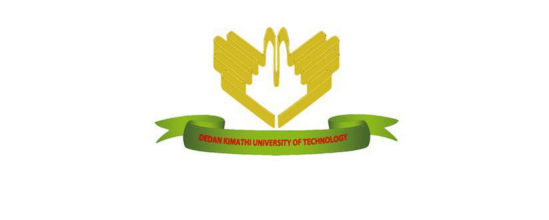
\includegraphics[width=0.5\textwidth]{dekut.png}
		
		\vspace{1cm}
		{\scshape\LARGE Dedan Kimathi University of Technology\par}
		\vspace{1cm}
		{\scshape\Large Bachelor of Science in Mathematics and Modeling Processes\par}
		\vspace{1.5cm}
		{\huge Comparing Local Outlier Factor and Random Forest Algorithms for Anomaly Detection in Raw Water Quality\par}
		\vspace{1cm}
		{\large\itshape NAME: KENNEDY WAMBUGU KINYUA\\REG: S084-01-2296/2021\par}
		\vfill
		\large \textbf{A research proposal submitted to the department of mathematics and physical science in partial fulfillment of requirement for award of the bachelor degree in bachelor of science in mathematics and modeling processes.}
\end{titlepage}


\linespread{1.5}
\pagenumbering{roman}
\begin{titlepage}
%\center
\Large \textbf{DECLARATION}\\[0.5cm]
\center 
\large DECLARATION BY THE STUDENT\\
%\large \textbf{Subject code} \\[0.5cm]
\paragraph{I declare that the work contained in this research proposal is my original work
and has not been presented for examination in any other University or
institution of higher learning.}

\begin{tabular}{p{0.4\linewidth}p{0.5\linewidth}}
  \textbf{Name: Kennedy wambugu kinyua} \\
  \vspace{12pt}
  signature: \dotfill & \vspace{12pt}  Date: \dotfill \\
\end{tabular}
\smallskip
%\left
\large DECLARATION BY THE SUPERVISOR\\
Department of Mathematics and Physical Sciences \\
\begin{tabular}{p{0.4\linewidth}p{0.5\linewidth}}
  \textbf{Name: MR. Rodgers  Amenya} \\
  \vspace{12pt}
  signature: \dotfill & \vspace{12pt}  Date: \dotfill \\
\end{tabular}
%\textbf{\large \today}
\end{titlepage}



%\newacronym{fpga}{FPGA}{Field Programmable Gate Array}
\newacronym{OSI}{OSI}{Open Standard Interface}
\newacronym{VHSIC}{VHSIC}{Very High Speed Integrated Circuit}
\newacronym{VHDL}{VHDL}{VHSIC Hardware Description Language}
\newacronym{VGA}{VGA}{Video Graphics Array}
\newacronym{bpp}{bpp}{bits per pixel}
\newacronym{TTL}{TTL}{Transistor Transistor Logic}
\newacronym{DTE}{DTE}{Data Terminal  Equipment}
\newacronym{DCE}{DCE}{Data Circuit Equipment}
\newacronym{USB}{USB}{Universal Serial  Bus}
\newacronym{UART}{UART}{Universal  Asynchronous Receiver/ Transmitter}
\newacronym{EIA}{EIA}{Electronic  Industries Alliance}
\newacronym{VDD}{VDD}{Voltage Drain Drain}
\newacronym{HSYNC}{HSYNC}{Horizontal Synchronization}
\newacronym{VSYNC}{VSYNC}{Vertical Synchronization}
\newacronym{IP}{IP}{Intellectual Property}
\newacronym{ISE}{ISE}{Integrated Synthesis Environment}
\newacronym{LSB}{LSB}{Least Significant Bit}
\newacronym{MSB}{MSB}{Most Significant Bit}
\newacronym{DAC}{DAC}{Digital to Analog Converter}
\newacronym{FIFO}{FIFO}{First In First Out}
\newacronym{LUT}{LUT}{Look Up Table}
\newacronym{ASIC}{ASIC}{Application Specific Integrated Chip}
\newacronym{IC}{IC}{Integrated Chip}
\newacronym{uart}{UART}{Universal Asynchronous Receiver and Transmitter}
\newacronym{RGB}{RGB}{Red Green Blue}
\newacronym{RAM}{RAM}{Random Access Memory}
\newacronym{XST}{XST}{Xilinx Synthesis Tool}
\newacronym{DDR SDRAM}{DDR SDRAM}{Double data rate synchronous dynamic random-access memory}
\newacronym{RTL}{RTL}{Register Transfer Language}

\subsection*{DEDICATION}
\addcontentsline{toc}{section}{DEDICATION}
\par
This research proposal is dedicated to my loving parents (Richard K. Wambugu \& Esther A. Kinyua) and siblings
for their moral support, financial assistance, encouragement, as well
as their self-denial and desire to ensure that I succeed and that the
department of mathematics and physical sciences for enabling me
to pursue this course.
\par

\clearpage

\subsection*{ACKNOWLEDGEMENT}
\addcontentsline{toc}{section}{ACKNOWLEDGEMENT}
First and foremost, I would want to express my gratitude to the
Almighty for the wisdom, knowledge, and spirit of persistence He
has bestowed upon me during my academic journey. I would like
to convey my heartfelt appreciation to my supervisor, Mr. Rogers
Amenya, for his devotion and commitment to ensuring I complete
an excellent research proposal. I am grateful to Center for Data
Science and Artificial Intelligence (DSAIL) in the Dedan Kimathi
University of Technology (DeKUT) team, their director Dr. Ciira
wa Maina, DeKUT, and Nahshon Mokua Obiri, for their mentorship,
inspiration, support with resources in my proposal  from Nyeri Water
and Sanitation Company (NYEWASCO) water quality laboratory.
\clearpage

%\subsection*{Acknowledgment}
%\addcontentsline{toc}{section}{Acknowledgment}
%\par
%\clearpage

\renewcommand{\sectionname}{}
\renewcommand\thesection{\arabic{section}}
\subsection*{\centering ABSTRACT}
\par
The increased use of real-time water quality monitoring using
automated systems with sensor demands and make it
possible to identify unexpected values in time. Anomalies are
brought by technical issues that are likely to prevent detection
of problematic data manually at the incoming data rate. Use of
machine learning approaches to detect anomalies in water
quality data is the main focus of this article. There is analysis
of three t machine learning anomaly detection
techniques: the local outlier factor, the isolation forest, and robust random cut forest. A subset of data collected from the deployment of sensors in a water
treatment plant (Nyeri-Kenya) will used to carry out extensive
analysis of experiments of the afore-mentioned techniques;
for turbidity and pH parameters.
\addcontentsline{toc}{section}{ABSTRACT}
\clearpage

\tableofcontents
\addcontentsline{toc}{section}{Table of contents}
\clearpage
\section*{ACRONYMS \& SYMBOLS}
\addcontentsline{toc}{section}{ACRONYMS \& SYMBOLS}
%\begin*{itemize}
    \item \textbf{LOF}: Local Outlier  Factor
    \item  \textbf{RRCF}: Random Robust  Cut  Forest. 
    \item \textbf{IF}: Isolation Forests.
    \item \textbf{DSAIL}: Center of  Data Science and  Artificial Intelligence. 
    \item  \textbf{NYEWASCO}:  Nyeri Water
And Sanitation Company. 
    \item \textbf{DeKUT}: Dedan Kimathi University  of  Technology.
%\end{itemize}
\clearpage

\begin


\pagenumbering{arabic}


\section*{\centering CHAPTER ONE}
 \addcontentsline{toc}{section}{CHAPTER ONE: INTRODUCTION}
\section*{\centering INTRODUCTION }
\counterwithin{subsection}{section} % Reset subsection numbering within each section
\setcounter{section}{1} % Set the section counter to 2 (since it starts from 0)
\setcounter{subsection}{-1}
\subsection{\centering INTRODUCTION & BACKGROUND INFORMATION}
\par
The interaction between human activities and the environment yields diverse effects, significantly impacting human health. Particularly, the growth of numerous slums, poor sanitation, and post-mining effects have disproportionately affected developing countries, contributing to environmental deterioration. In response, global initiatives have been established to promote ecological sustainability through environmental monitoring programs. Notably, air quality monitoring systems have been implemented by governments and international organizations as part of this effort, with proposals for water quality monitoring systems, and advancements in animal tracking for environmental sustainability.

Water, a fundamental resource for life, covering over 70\% of the Earth's surface, is crucial for survival. However, ensuring water quality presents challenges due to its complex network comprising various interconnected components such as lakes, rivers, creeks, estuaries, and wetlands. Fluctuating pollution levels across these components pose difficulties in assessing water quality.

Water quality encompasses chemical, physical, biological, and other constituents that vary based on seasons and geographical locations. Environmental factors and human activities significantly influence water quality, with climate, geological, and hydrological factors being primary determinants. Human activities impact water quality extensively, affecting both human and environmental health. Hence, constant monitoring of water quality is essential for identifying and preventing contamination issues.
\par
Anomalies in water quality analysis, often caused by ecological phenomena like floods or rainfall, as well as human and technical errors, can lead to erroneous decisions and conclusions. These errors may stem from communication breakdowns between servers and sensor nodes, sensor probe contamination, and equipment malfunctioning, among other factors.
This research proposal seeks to build upon these foundations by further investigating advanced anomaly detection techniques and leveraging emerging technologies in data science and artificial intelligence to enhance the accuracy and efficiency of water quality monitoring systems. By refining anomaly detection algorithms and incorporating real-time data analytics, the proposed research aims to contribute to the sustainable management of water resources and the protection of human and environmental health.
\subsection{STATEMENT OF THE PROBLEM}
\par
Traditional statistical methods for anomaly detection often fall short when dealing with high-dimensional, non-linear, and dynamic data streams. Machine learning algorithms, on the other hand, offer a powerful and flexible approach to tackle this challenge. By leveraging advanced techniques such as density-based methods, isolation forests, and ensemble models, machine learning algorithms can learn the intrinsic patterns and characteristics of normal data, enabling them to effectively distinguish anomalies from regular observations. However, the efficacy of these algorithms varies across different domains and data distributions, necessitating a comprehensive evaluation and comparison of their performance on real-world water quality datasets.
\par
The  machine learning anomaly detection algorithms: Local Outlier Factor (LOF), Isolation Forest (IF) and  (RRCF) Robust
random cut forest. These algorithms are evaluated on a subset of water quality data collected from a water treatment plant, focusing on two critical parameters: turbidity and pH. The aim is to identify the most effective and efficient algorithm for detecting anomalies in real-time water quality data streams, taking into account factors such as accuracy, computational complexity, and scalability. By addressing this problem, the research contributes to the development of reliable and robust anomaly detection systems, enabling timely intervention and proactive maintenance in water quality monitoring applications.

\subsection{JUSTIFICATION}
\par
Water quality monitoring is a critical aspect of environmental protection and public health. The increasing deployment of automated sensor networks for real-time water quality monitoring generates vast amounts of data. However, the presence of anomalies or outliers in this data, caused by factors such as equipment malfunctions, environmental changes, or human errors, can lead to inaccurate analyses and flawed decision-making processes. Failing to detect and address these anomalies promptly can have severe consequences, including potential health hazards and environmental degradation. Traditional statistical methods may not be sufficient for accurately identifying anomalies in complex, high-dimensional, and dynamic data streams. Therefore, there is a pressing need for robust and efficient machine learning algorithms that can learn the intrinsic patterns of normal data and effectively detect anomalies in real time. The research paper addresses this crucial issue by conducting a comprehensive evaluation and comparison of four prominent machine learning anomaly detection algorithms on real-world water quality data. By identifying the most effective and efficient algorithm, the study contributes to the development of reliable anomaly detection systems, enabling timely intervention, proactive maintenance, and ultimately safeguarding water resources and public health.
\subsection{OBJECTIVES}
\subsubsection{Main objective}
\begin{itemize}
    \item By identifying the most effective and efficient algorithm, the study contributes to the development of reliable anomaly detection systems.
\end{itemize}
\subsubsection{Specific objective}
\begin{itemize}
    \item To evaluate and compare two ML anomaly detection algorithms (LOF, IF, RRCF) on real water quality data.
\item To identify the most effective and efficient algorithm for detecting anomalies in real-time water quality data.
\item To provide valuable insights to enhance water quality management procedures to guarantee the security of water sources.
\end{itemize}
\subsection{Assumptions}
\begin{enumerate}
    \item The data collected from sensors is accurate, reliable, and representative of the actual water conditions.
\item  The results and conclusions drawn from the study can be generalized to similar water quality monitoring scenarios and datasets.
\item Optimal parameter settings for the algorithms can be determined effectively.
\end{enumerate}
\subsection{Limitations}
\begin{enumerate}
    \item Limitations in the computational resources necessary for deploying machine learning algorithms.
\item Presumptions established during data preprocessing and fine-tuning of algorithm parameters.
\item  How well the results can be used for other types of water quality monitoring and data.
\end{enumerate}

\subsection{Scope of the  study}
\begin{itemize}
    \item Evaluation of the LOF algorithm and Random Forest algorithms for anomaly detection in raw water quality data.
\item Comparison of different machine learning techniques for real-time monitoring of water contamination.
Optimization of algorithm parameters to enhance accuracy and efficiency in anomaly detection.
\item Contribution of insights to enhance water quality management practices and ensure the safety of water sources.
\end{itemize}

\clearpage

\section*{\centering CHAPTER TWO}
\subsection*{\centering LITERATURE  REVIW}
%\addcontentsline{toc}{section}{CHAPTER TWO}
\addcontentsline{toc}{section}{CHAPTER TWO:LITERATURE REVIEW}
\counterwithin{subsection}{section} % Reset subsection numbering within each section
\setcounter{section}{2} % Set the section counter to 2 (since it starts from 0)
\setcounter{subsection}{-1}
%\subsection{\centering LITERATURE REVIEW}
\par
\subsubsection{Machine learning for anomaly detection and process phase
classification to improve safety and maintenance activities(Elena Q, R. Patriarca (2020)}
The paper "Machine Learning for Anomaly Detection and Process Phase Classification in Industrial Processes" \cite{ml_paper1} introduces an innovative methodology that combines machine learning algorithms to process phase identification to enhance anomaly detection in industrial settings facing dynamic operational conditions. By addressing the limitations of traditional signal processing techniques in such environments, the study underscores the crucial role of domain experts in delineating normal and abnormal behavior boundaries and extracting valuable insights from complex data. Through a detailed case study in the pharmaceutical industry, the paper showcases the practical utility and effectiveness of the proposed approach, achieving impressive results in anomaly detection. The research not only emphasizes the importance of real-time implementation but also highlights the need for continuous algorithm parameter updates to adapt to changing industrial landscapes.

\subsubsection{An integrated data-driven framework for surface water quality anomaly detection and early warning (Jie LiuPeng WangPeng WangDexun Jiang(2019))}
\par
The paper "An integrated data-driven framework for surface water quality anomaly detection and early warning" \cite{paper2} focuses on the importance of detecting anomalies in surface water quality to prevent harmful compounds from spreading due to environmental spills or intentional releases into rivers. A data-driven framework is developed for early warning detection of surface water quality anomalies, crucial for addressing river pollution in advance. The framework combines a Bayesian autoregressive (BAR) model for predicting water quality variations and an Isolation Forest (IF) algorithm for anomaly detection. Firstly, the BAR model predicts water quality variations using Bayesian inference. Then, the IF algorithm identifies anomalies by analyzing prediction residuals. The framework is applied to analyze and detect surface water quality variations and anomalies in the Potomac River, West Virginia, USA. Comparative analysis with other methods and scenarios demonstrates that the integration framework not only improves anomaly detection accuracy but also enables quick response for emergency operations.
\subsubsection{Robust random cut
forest based anomaly detection on streams (S. Guha, N. Mishra, G. Roy and O. Schrijvers(2016))}
\par
In the paper "Robust Random Cut Forest Based Anomaly Detection On Streams," \cite{paper3} the authors delve into the realm of anomaly detection in dynamic data streams using random cut forests. By proposing a robust data structure to encapsulate the input stream and introducing a novel definition of non-parametric anomalies based on the impact of unseen points, the study sheds light on the intricate process of identifying anomalies in evolving data environments. The algorithm's ability to adapt efficiently to changes in the data stream, including corrections and updates, showcases its practical relevance in real-world scenarios. Overall, the research contributes significantly to the field of anomaly detection by offering a fresh perspective on model complexity and dynamic data structures, paving the way for enhanced anomaly detection methodologies in streaming data applications.
\subsubsection{OF: Iden-
notifying Density-Based Local Outliers (M. M. Breunig, H.-P. Kriegel, R. T. Ng and J. Sander(2000))}
The paper by Breunig et al\cite{paper4}. introduces the concept of the local outlier factor (LOF) for outlier detection in datasets, emphasizing the importance of considering the degree of outlying ness for each object rather than a binary outlier classification. Through a detailed analysis of LOF properties and experimental validation, the authors demonstrate the effectiveness of LOF in identifying local outliers that traditional methods may miss. They provide insights into the impact of parameters like MinPts on LOF values and offer practical guidelines for selecting appropriate values. Overall, the paper contributes a valuable perspective on outlier detection, showcasing the significance of a local approach in uncovering meaningful outliers in complex datasets.
\subsubsection{Anomaly Detection: A Survey (Varun Chandola, Arindam Banerjee, and Vipin Kumar(2007))}
In their comprehensive survey on anomaly detection \cite{paper5}, Chandola, Banerjee, and Kumar delve into the intricate challenges and diverse applications of identifying patterns that deviate from expected normal behavior. They highlight the complexity of defining normal regions and the evolving nature of anomalies, emphasizing the difficulty in distinguishing between noise and true anomalies. By categorizing techniques into six distinct groups and discussing unique assumptions underlying each approach, the authors offer a structured overview that expands upon existing works. Their exploration of complex anomalies in various domains sheds light on the gap between algorithmic research focusing on simple anomalies and the nuanced anomalies prevalent in real-world scenarios. This survey not only contributes a broad perspective on anomaly detection techniques but also provides valuable insights for future research and practical implementations.
\clearpage 
\section*{\centering CHAPTER THREE}
\subsection*{\centering RESEARCH METHODOLOGY}
 \addcontentsline{toc}{section}{CHAPTER THREE:RESEARCH METHODOLOGY}
\counterwithin{subsection}{section} % Reset subsection numbering within each section
\setcounter{section}{3} % Set the section counter to 2 (since it starts from 0)
\setcounter{subsection}{-1}
\subsection{Data Collection}
\begin{itemize}
    \item \textbf{Data Collection}: Subset data collected from sensors deployed in a water treatment plant in Nyeri, Kenya.
\end{itemize}
\subsection{Model Selection: Anomaly Detection Algorithms}
\begin{enumerate}
  \item  \textbf{Local Outlier Factor Algorithm:}
  \par
 It is an algorithm used for Unsupervised outlier detection. It produces an anomaly score that represents data points that are outliers in the data set.
\par  
Parameters  used: 
k: The distance between the k-th neighbor. 
Reachability  Distance
Local Outlier  Factor
Local Reachability  Distance
\par  
\begin{flushleft}
Maths  behind \textbf{LOF} : \\ 
\begin{enumerate}
    \item k: Number of neighbors. (user-defined) \\
\item Reachability  Distance(a,b):\begin{equation}
   Reachability  Distance(a,b) =  max(distance(b), normal\_distance(b))
\end{equation}
\item Local Reachability Distance: \begin{equation}
    Local Reachability Distance(a)  = \frac{\frac{1}{\sum reachability distance(a,n)}}{k}
\end{equation}
where n is neighbors up to k.
\end{flushleft}
\item  \textbf{LOF}:
\begin{equation}
    LOF(a)  = \frac{\frac{[LRD(1^{st} neighbour) + LRD(2^{nd} neighbour) +...LRD(n^{th} neighbour)]}{LRD(a)}}{k}
\end{equation}
\end{enumerate}
\clearpage
  \par
 This distance is used to calculate the reachability distance, see figure \ref{fig: lof}. It is defined as the maximum distance between two points and the k-distance of that point.
 \begin{figure}[h]
    %\centering
    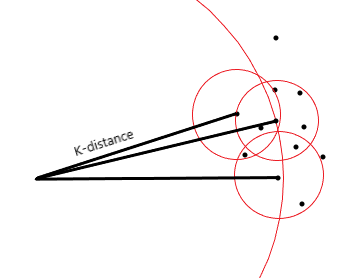
\includegraphics[width=0.5\linewidth]{lof.png}
    \caption{Local factor  algorithm k-distance illustration}
    \label{fig:lof}
\end{figure}
\clearpage
\item  \textbf{Isolation Forest:}
\par
Isolation forest is a state-of-the-art anomaly detection algorithm famous for its efficiency and simplicity, see \ref{fig:if}. Removing anomalies from a dataset using binary partitioning quickly identifies outliers with minimal computational overhead, making it the way to go for anomaly detection.
\par
How  it  works: \\
\par
When given a dataset, a random subsample of the data is selected and assigned to a binary tree.
\begin{enumerate}
    \item Branching of the tree starts by selecting a random feature (from the set of all N features) first. Then branching is done on a random threshold (any value in the range of minimum and maximum values of the selected feature).

\item  If the value of a data point is less than the selected threshold, it goes to the left branch or to the right. And thus a node is split into left and right branches.
\end{enumerate}
\par
 This process from step 2 is continued recursively till each data point is completely isolated or till max depth (if defined) is reached.
 \par 
 Math Behind the  Isolation Forest: 
 For  the  scores: \\ 
 $ s(x,m)  = 2^{-{\frac{E(h(x))}{c(m)}}} $
 Where: \\ 
 $ m = $ Number of points. \\ 
$ x  = $ Data point.  \\
$ E(h(x)) $ = Average or expected average path for isolating data point x. \\
Where  if:\\
\\
$E(h(x)) <  (c(m)  \implies s(x,m) \approx 1 $ \\
$E(h(x))   = c(m) \implies s(x,m) \approx 0 $ \\
$E(h(x)) > c(m) \implies s(x,m) \approx -1 $\\


\begin{figure}[h]
    \centering
    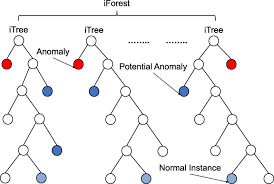
\includegraphics[scale =0.5]{iso.png}
    \caption{Isolation Forest}
    \label{fig:if}
\end{figure}
\clearpage
\item \textbf{Robust
random cut forest:}
This anomaly detection algorithm on streaming data was
proposed in 2016 \cite{paper3}. 
\begin{enumerate}
    \item A bunch of random instances is taken by RRCF
(Random).
\item It then cuts them into the same number of instances
and creates trees (Cut).
\item Finally, all the trees together are considered by
determining whether a particular instance is an
anomaly (Forest).
\end{enumerate}
\par

On a point set $S$, a robust random cut tree (RRCT) is generated as follows:
\begin{enumerate}
    \item A random element relational to $\frac{l_i}{\sum l_j}$ where $l_i = \max_{x \in S} x_i - \min_{x \in S} x_i$ is chosen.
    \item Choose $X_t \sim \text{Uniform}[\min_{x \in S} x_i, \max_{x \in S} x_i]$
    \item Let $S1 = \{ x \mid x \in S, x_i \leq X_t \}$, $S2 = S / S1$ and recurse on $S1$ and $S2$
\end{enumerate}

The figure below\ref{fig:randomcut} shows how RRCF cut instance happens into pieces
recursively. When each point is isolated, the cutting is
stopped.  \\
\begin{figure}[h]
    \centering
    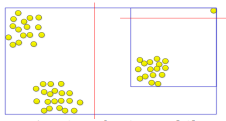
\includegraphics[scale =0.5,]{random_cut.png}
    \caption{Random cut forest  illustration}
    \label{fig:randomcut}
\end{figure}
\end{enumerate}
\par
The  methodology is represented by the block diagram: \\
\begin{figure}[h]
    %\centering
    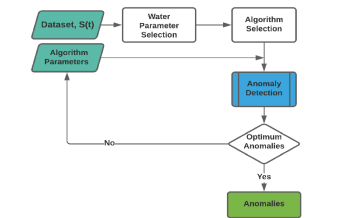
\includegraphics[width=0.5\textwidth]{methodology.png}
    \caption{Flow  Chart  Diagram}
    \label{fig:methods}
\end{figure}
\clearpage
\subsection{Expected  Outcome}
The anticipated results of the study include the successful detection of anomalies in raw water quality data using the Local Outlier Factor (LOF) algorithm, Isolation Forest (IF), and  Robust
random cut forest  (RRCF). The study aims to compare the performance of these algorithms in detecting outliers, optimizing parameters for improved accuracy, assessing feasibility for real-time monitoring, and contributing valuable insights to the field of water quality monitoring.

\clearpage 
\section*{\centering CHAPTER FOUR}
\addcontentsline{toc}{section}{CHAPTER FOUR:RESULTS}
\subsection*{\centering RESULTS  AND  DISCUSSION}
\counterwithin{subsection}{section} 
\setcounter{section}{4}
\setcounter{subsection}{-1}

This chapter presents the findings of the research on anomaly detection in raw water quality data using three machine learning algorithms: Local Outlier Factor (LOF), Isolation Forest (IF), and Robust Random Cut Forest (RRCF). The performance of each algorithm was evaluated based on their ability to detect anomalies in the turbidity and pH levels of water collected from sensors deployed at the Nyeri Water Treatment Plant in Kenya. The results are analyzed and discussed, determining the most effective algorithm for real-time water quality monitoring.
\subsection{Overview of the Dataset}
The data used in this study was collected over a period of time  of 
 30 mins  interval from the Nyeri Water Treatment Plant. The dataset includes measurements of \textbf{turbidity} and  \textbf{pH} water quality parameters,  as key indicators of water quality.
 The data was preprocessed:
 \subsection{Data preprocessing}
 \par  
 The  data  contained  2658 rows  and  3  columns, that  is \textbf{Turbidity}, \textbf{pH}, \textbf{time}. Turbidity  refers, how cloudy or hazy a fluid is due to suspended particles that scatter (measured  in Nephelometric Turbidity Units (NTU)), pH refers  to  a measure of how acidic the  water  is while  time  is  the  interval of  when  the  data  was  collected,$$\approx \text{32 minutes from the  water  sensors.} $$

 \begin{figure}[h]
     \centering
     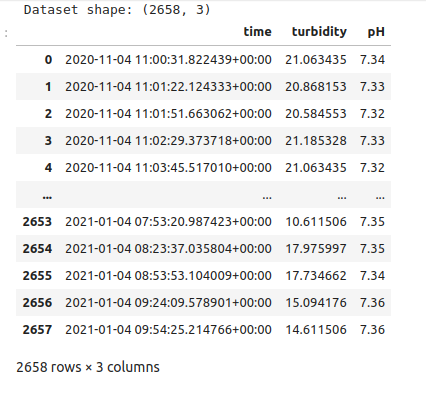
\includegraphics[scale = 0.3]{dataset.png}
     \caption{Dataset  overview}
     \label{fig:enter-label}
 \end{figure}
\par
The  trends  of  each variable  over  the  time  was:\\


\begin{figure}[h]
    \centering
    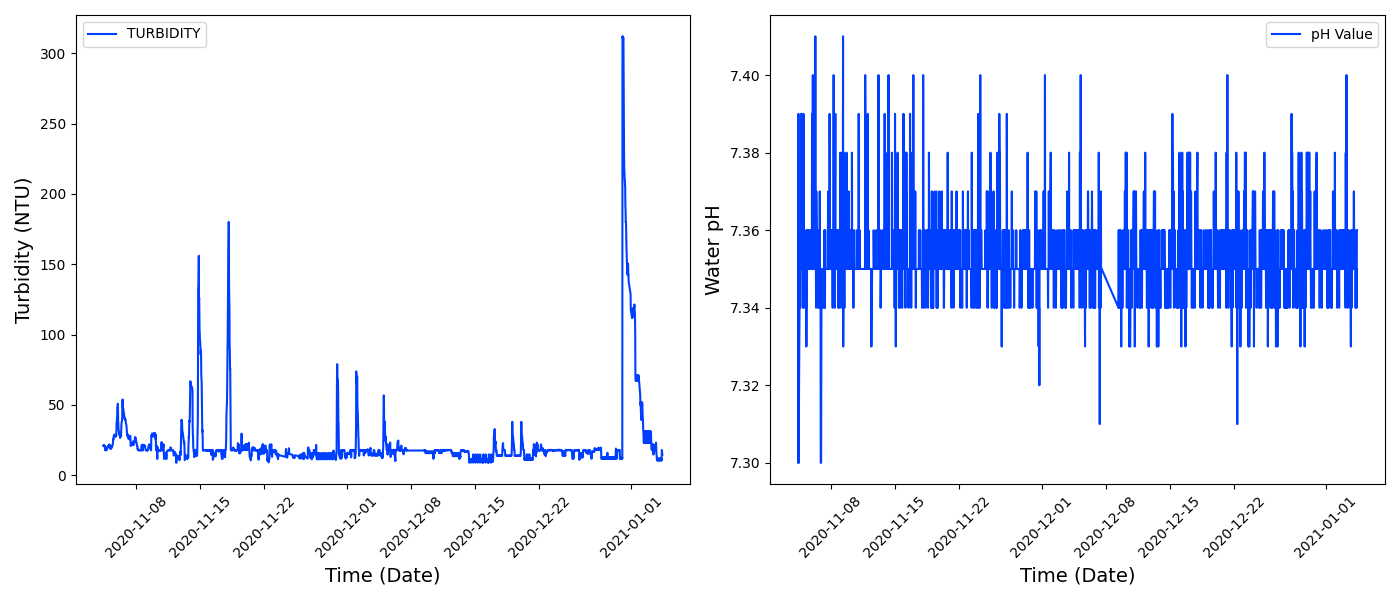
\includegraphics[width=0.5\linewidth]{vaiables_trend.png}
    \caption{Variable  trends ie  turbidity  and  pH}
    \label{fig:enter-label}
\end{figure}

Turbidity Plot:
\begin{enumerate}
 \item Baseline: The turbidity generally remains low, mostly below 50 NTU (Nephelometric Turbidity Units).

 \item Spikes: 
   - A few smaller spikes in the middle, around 30-160 NTU.
   - A very large spike near the end, exceeding 300 NTU.
Outside the spikes, there's some minor fluctuation in the baseline turbidity.
These trends suggest:
\begin{itemize}
    \item Generally clear water, with occasional events causing temporary increases in suspended particles.
    \end{itemize}
\end{enumerate}
pH Plot:
\begin{enumerate}
    \item  Range: The pH values mostly fluctuate between 7.32 and 7.40, indicating slightly alkaline water.
\item  Stability: Overall, the pH is relatively stable, with no extreme fluctuations.
\item  Pattern: There are frequent small variations within this narrow range.
\end{enumerate}
These trends suggest:
\begin{itemize}
    \item  The water source maintains a consistent, mildly alkaline pH.
    \item Small variations could be due to natural factors or minor changes in water chemistry.
    \tem The stability indicates a well-buffered system resistant to major pH changes.
\end{itemize}
In summary, the water quality shows stable pH levels with occasional turbidity events. The pH remains consistently in a healthy range for most use  cases, while the turbidity data suggests the water is generally clear but subject to periodic increases in suspended particles, likely due to environmental events or human activities.
\clearpage
\subsubsection{Variable  distribution}
\begin{figure}[h]
    \centering
    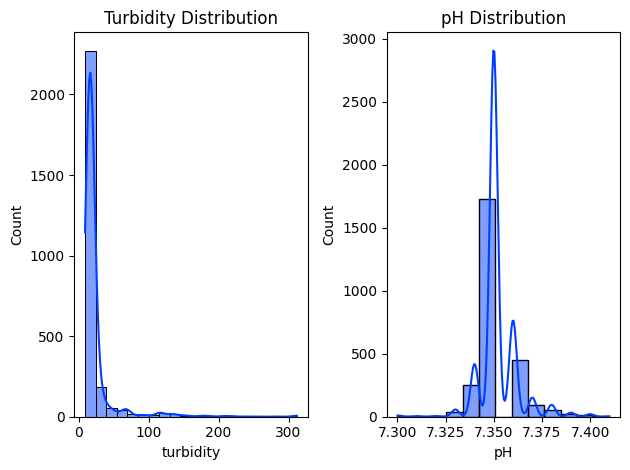
\includegraphics[width=0.5\linewidth]{distribution.png}
    \caption{variables  distribution Distribution}
    \label{fig:enter-label}
\end{figure}
    
\subsubsection{Turbidity Distribution}
\begin{itemize}
    \item \textbf{Shape}: The turbidity distribution is highly right-skewed (positively skewed). Most of the data points are concentrated at the lower end of the scale.
    \item \textbf{Concentration}: A significant number of observations have very low turbidity values, close to zero.
    \item \textbf{Outliers}: There are a few observations with much higher turbidity values, extending up to around 300, but these are relatively rare.
\end{itemize}
\subsubsection{pH Distribution}
\begin{itemize}
    \item \textbf{Shape}: The pH distribution is approximately normal but with a very narrow range.
    \item \textbf{Concentration}: The majority of the pH values are tightly clustered around the mean, which appears to be around 7.35.
    \item \textbf{Spread}: The distribution shows a high peak, indicating that most of the pH values are very close to the mean, with very few values deviating significantly from it.
\end{itemize}

\subsubsection*{Insights}
\begin{enumerate}
    \item \textbf{Turbidity}: The data suggests that most samples have low turbidity, indicating clear water in most cases. However, there are occasional instances of high turbidity, which could be due to specific events or conditions causing temporary increases in water turbidity.
    \item \textbf{pH}: The pH values are very consistent and centered around a neutral pH of 7.35. This indicates stable water quality in terms of acidity and alkalinity, with very little variation.
\end{enumerate}

 \newpage
 \subsection{Model  Performance}
\subsubsection{Anomaly Detection with Local Outlier Factor (LOF)}
The LOF algorithm was applied to the dataset to identify local anomalies in the turbidity and pH levels. LOF assigns an anomaly score to each data point based on its distance from its neighbors. The results indicated that LOF was effective in detecting small clusters of anomalies that might indicate localized issues in water quality.
Parameter  tuning  was  done  using  GridSearchCV  method to find  the  best  combination of  the  parameters. 

\begin{figure}[h]
    \centering
    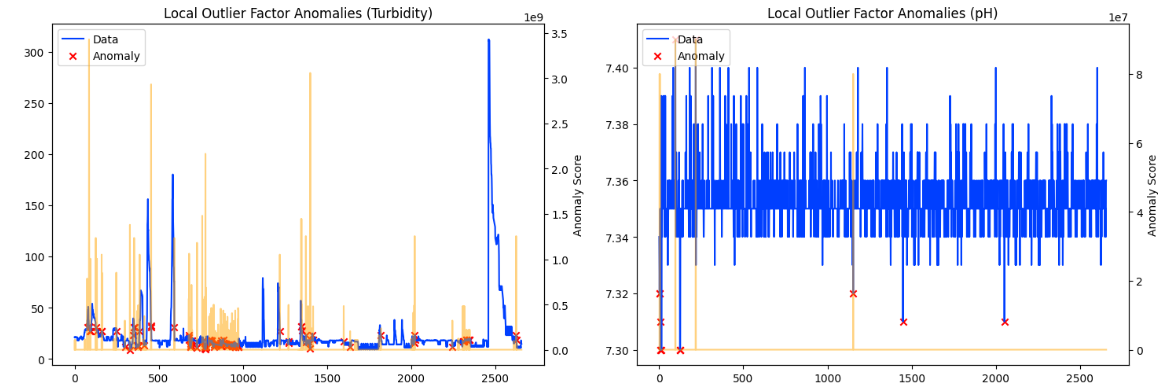
\includegraphics[width=1 \linewidth]{lof_performance.png}
    \caption{LOF anomaly performance for pH  and  Turbidity  variables.}
    \label{fig:enter-label}
\end{figure}
\subsubsection{Local Outlier Factor (LOF) Algorithm}

\begin{enumerate}
    \item \textbf{Principle}: LOF compares the local density of a point to the local densities of its neighbors. Points that have a substantially lower density than their neighbors are considered outliers.
    
    \item \textbf{Parameter Tuning}: The parameters like the number of n\_neighbors (k) were optimized to find the best configuration for anomaly detection.
\end{enumerate}

\subsubsection{Analysis of Turbidity Anomalies}

\begin{enumerate}
    \item \textbf{Sensitivity}: The LOF algorithm appears highly sensitive to turbidity fluctuations, detecting numerous anomalies throughout the time series.

    \item \textbf{Major Spikes}: The algorithm failed to  identify major turbidity spikes, particularly the large spike near the end of the series (around data point 2500) where turbidity exceeds 300 NTU.

    \item \textbf{Moderate Anomalies}: Several moderate spikes (around 150-200 NTU) are also not  flagged as anomalies, indicating the algorithm's ability to detect less extreme but still significant deviations.
\end{enumerate}
\subsubsection{Analysis of pH Anomalies}

\begin{enumerate}
    \item \textbf{Narrow Range}: Despite the pH values fluctuating within a narrow range (approximately 7.30 to 7.40), the LOF algorithm still detects anomalies.

    \item \textbf{Sensitivity to Slight Changes}: The algorithm identifies anomalies even for small deviations in pH, highlighting its sensitivity to local density variations in tightly clustered data.

    \item \textbf{Fewer Anomalies}: Compared to turbidity, there are fewer detected anomalies in pH, which aligns with the overall stability of pH values.

    \item \textbf{Extreme Values}: The most prominent anomalies in pH correspond to the lowest values in the series (around 7.30-7.32), and  (around 7.38-7.40).
\end{enumerate}
This  shows  that LOF  did not adapt well in identifying  anomalies  in this  case  senario.
\subsubsection{Isolation Forest Algorithm Overview}
The Isolation Forest is an unsupervised learning algorithm designed to detect anomalies.
\begin{enumerate}

    \item \textbf{Parameter Tuning}: The parameters like the number of n\_estimators, max\_samples, contamination were optimized to find the best configuration for anomaly detection using  gridsearchcv. 
\end{enumerate}

\begin{figure}[h]
    \centering
    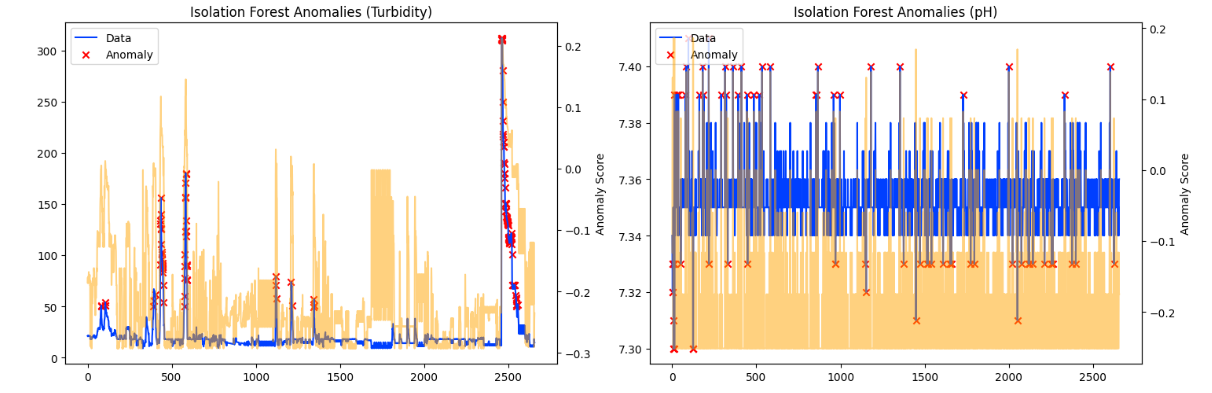
\includegraphics[width=1 \linewidth]{isolatio_forest_model.png}
    \caption{Isolation forest  model}
    \label{fig:enter-label}
\end{figure}
\subsubsection*{Performance Analysis}
\subsubsection{Turbidity Anomaly Detection}
\begin{itemize}
    \item \textbf{Spike Detection:} The algorithm successfully captured the most significant turbidity spikes, particularly the large spike near the end of the time series (around data point 2500) where turbidity exceeds 300 NTU.
    \item \textbf{Moderate Anomalies:} It also identified several moderate spikes that  are  visible  as  anomalies in the  visualization. 
    \item \textbf{Baseline Sensitivity:} The algorithm appears less sensitive to minor fluctuations in the baseline turbidity compared to the LOF method, focusing more on significant deviations, in which in real life  relates  to affect  water  quality most. 
    \item \textbf{Cluster of Anomalies:} A dense cluster of anomalies is detected during the major turbidity event at the end, indicating the algorithm's ability to flag sustained anomalous behavior.
\end{itemize}

\subsubsection{pH Anomaly Detection}
\begin{itemize}
    \item \textbf{Range Sensitivity:} Despite the narrow range of pH values (approximately 7.30 to 7.40), the Isolation Forest detected numerous anomalies.
    \item \textbf{Extreme Values:} The algorithm consistently identified the lowest and highest pH values as anomalies.
    \item \textbf{Balanced Detection:} Anomalies are detected throughout the pH range, suggesting good sensitivity to both high and low extremes.
    \item \textbf{Frequency:} The number of anomalies detected in pH is higher than in turbidity, possibly due to the algorithm's sensitivity to slight variations in a tightly clustered dataset.
\end{itemize}

%\subsection{Comparative Performance}
\subsubsection{Turbidity}
The Isolation Forest seems more selective in identifying turbidity anomalies compared to the LOF method, focusing on more significant deviations.

\subsubsection{pH}
For pH, the Isolation Forest appears to be highly sensitive, detecting numerous anomalies despite the narrow value range.

\subsubsection{Suitability for Tracking Anomalies}
\begin{itemize}
    \item \textbf{Adaptability:} The algorithm demonstrates good adaptability across different scales of data (wide-ranging turbidity vs. narrow-range pH).
    \item \textbf{Focus on Extremes:} It effectively highlights extreme values, which is crucial for water quality monitoring.
    \item \textbf{Reduced Noise:} Especially for turbidity, it seems to reduce false positives from minor fluctuations, focusing on more significant anomalies.
    \item \textbf{Sensitivity Tuning:} The use of grid search CV for parameter tuning likely contributed to optimizing the algorithm's performance for this specific dataset.
\end{itemize}


\subsubsection{RRCF Detection of Anomalies in Turbidity}
\begin{itemize}
    \item \textbf{Spike Detection:} The left plot displays the anomaly detection in turbidity levels. The red 'x' markers indicate where the RRCF algorithm detected anomalies. The algorithm successfully identifies significant spikes, particularly around the data points between 0-500 and 2500-2750. However, the RRCF seems to miss some of the smaller spikes that were captured in the earlier Isolation Forest model. This indicates that while the RRCF is robust, it might be slightly less sensitive to smaller, less prominent anomalies.
    \item \textbf{Smoothness in Anomaly Score:} The anomaly score appears smoother, with the algorithm providing a clearer distinction between normal and anomalous data. This could imply a better generalization by the RRCF in identifying truly abnormal events rather than just spikes.
\end{itemize}

\subsubsection{Detection of Anomalies in pH Levels}
\begin{itemize}
    \item \textbf{Consistency in pH Data:} The right plot shows the RRCF performance on pH levels. Here, the RRCF algorithm detects anomalies but appears to be more conservative than the previous Isolation Forest model. The anomaly scores are more spread out, and fewer anomalies are detected, which may indicate that the model is focusing on more significant deviations rather than minor fluctuations.
    \item \textbf{Anomaly Distribution:} The anomalies detected are distributed throughout the dataset, suggesting that the algorithm is tracking changes in the underlying pattern rather than just focusing on outliers. This is particularly useful in datasets like pH, where fluctuations may be frequent but not necessarily indicative of a true anomaly.
\end{itemize}

\subsection{Discussion}

The Robust Random Cut Forest algorithm has shown a strong capability in detecting anomalies, particularly in more structured and less volatile datasets like pH levels. Compared to the Isolation Forest algorithm, RRCF seems to provide a more nuanced understanding of what constitutes an anomaly, focusing on overall patterns rather than just spikes.

\subsubsection{Turbidity Data}
While RRCF effectively identifies major spikes, it seems to be slightly less sensitive to smaller anomalies. This might be due to its inherent design, which aims to balance robustness and sensitivity. For datasets where identifying every spike is critical, further tuning might be needed to improve sensitivity.

\subsubsection{pH Data}
RRCF performs well in detecting significant anomalies in the pH data, showing its strength in datasets where the anomalies are subtle and more pattern-based. The smoother anomaly score suggests that the algorithm is less prone to overfitting and might be more reliable in long-term monitoring.

\subsection{Suitability for Anomaly Detection}

\subsubsection{Turbidity Data}
The RRCF algorithm is suitable for tracking significant anomalies in turbidity data, especially where robustness and the avoidance of false positives are important. However, if the application requires the detection of every minor fluctuation, additional tuning may be necessary, it  is  not  suitable  for detection of  anoalies in the  water quality  monitoring.

\subsubsection{pH Data}
RRCF is particularly well-suited for pH data, where anomalies are less about spikes and more about changes in patterns. The algorithm’s ability to detect significant deviations while minimizing false positives makes it ideal for this type of data.
\par
Robust Random Cut Forest algorithm, provides a balanced approach to anomaly detection. It is especially effective in environments where a mix of sensitivity and robustness is required, though careful tuning is essential to align the model’s performance with the specific needs of the dataset.



\section*{Conclusion}
The Isolation Forest algorithm demonstrates strong performance in detecting anomalies in both turbidity and pH data. Its ability to capture significant spikes while potentially reducing noise in turbidity measurements, combined with its sensitivity to subtle changes in pH, makes it a suitable tool for tracking anomalies in water quality data. The algorithm's adaptability to different data characteristics, enhanced by parameter tuning through grid search CV, suggests it could be a valuable component in a comprehensive water quality monitoring system. However, the high sensitivity in pH detection might require careful threshold setting to distinguish between operationally significant anomalies and normal variations.

\subsection{Comparative Analysis of the Algorithms}
The three algorithms were compared based on their performance in detecting anomalies, computational efficiency, and suitability for real-time monitoring: \\
\begin{table}[h!]
\centering
\caption{Performance of Anomaly Detection Algorithms}
\resizebox{\textwidth}{!}{%
\begin{tabular}{|l|c|c|c|}
\hline
\textbf{Algorithm} & \textbf{Sum of Anomalies Detected} & \textbf{Sum of Anomalies Not Detected} & \textbf{Time Taken to Train Model (s)} \\ \hline
\textbf{Isolation Forest (Turbidity)} & 182 & 34 & 5.87 \\ \hline
\textbf{Local Outlier Factor (Turbidity)} & 0 & 216 & 0.28 \\ \hline
\textbf{Robust Random Cut Forest (Turbidity)} & 19 & 197 & 2.09 \\ \hline
\textbf{Isolation Forest (pH)} & 1719 & 0 & 5.64 \\ \hline
\textbf{Local Outlier Factor (pH)} & 58 & 1661 & 0.65 \\ \hline
\textbf{Robust Random Cut Forest (pH)} & 0 & 1719 & 32.62 \\ \hline
\end{tabular}%
}
\label{tab:algorithm_performance}
\end{table}



\clearpage
\subsection{Discussion}
A subset of data that was used in algorithm evaluation had 216 records for turbidity and  1819 for pH variables, extracted from the 2,658 that were collected over the
deployment period. The IF algorithm emerged superior to
the LOF and RRCF algorithms in contamination or
anomaly event detection, and hence a practical water
contamination detection algorithm that can trigger alarms to
alert the analyzers when contamination is detected. Moreover, the LOF, and the RRCF algorithms exhibited inconsistent results in   identifying  the extreme values.
The findings from this research highlight the strengths and limitations of each anomaly detection algorithm when applied to raw water quality data. IF algorithm  emerged  the best  in terms  of accurately  identifying  extreme  anomalies  and  efficiency in computing  efficiency.   
However, the choice of algorithm should be guided by the specific requirements of the monitoring system, including the nature of the data, the computational resources available, and the need for real-time detection. Combining these algorithms in a hybrid approach could potentially offer a more comprehensive solution for water quality monitoring.
\clearpage

\section*{\centering CHAPTER FIVE}
 \addcontentsline{toc}{section}{CHAPTER FIVE: CONCLUSIONS  AND  RECCOMENDITIONS}
\section*{\centering Conclusion and Recommendations}
\counterwithin{subsection}{section} % Reset subsection numbering within each section
\setcounter{section}{5} % Set the section counter to 2 (since it starts from 0)
\setcounter{subsection}{-1}
%\section{}{Conclusion and Recommendations}
\subsection{Conclusion}
This research has successfully evaluated and compared the performance of three machine learning algorithms—Local Outlier Factor, Isolation Forest, and Robust Random Cut Forest—in detecting anomalies in raw water quality data. The results demonstrate that each algorithm has its own strengths and weaknesses. 
IF algorithm  emerged the  best  in terms  of detecting  the  anomalies  with very  high spikes. \\
More water quality parameters can be subjected to the
analysis done besides turbidity and water pH; these include:
Total Dissolved Solids, Oxygen Reduction Potential,
Temperature, Electrical Conductivity, Dissolved Oxygen,
Free Residual Chlorine, Nitrates, to mention just but a few.
Additionally, more anomaly detection algorithms can be
assessed too to give a more robust and detailed report on
anomaly detection algorithms.
\begin{itemize}
    \item \textbf{Local Outlier Factor (LOF):} Best suited for detecting localized anomalies but requires careful parameter tuning.
    \item \textbf{Isolation Forest (IF):} Offers a balance between detection accuracy and computational efficiency, making it ideal for large-scale monitoring.
    \item \textbf{Robust Random Cut Forest (RRCF):} Provides the best adaptability to changing data patterns, making it the most reliable very little  flactuations  in the data.
\end{itemize}

The research concludes that no single algorithm is universally superior; the choice of algorithm should be based on the specific characteristics of the dataset and the operational requirements of the monitoring system, but  the  best  anomaly  detection algorithm to detect  anomalies  is  IF, it  has a  balance  between  computational efficiency  and  identifying  extreme  values. 

\subsection{Recommendations}
Based on the findings of this research, the following recommendations are made:

\begin{enumerate}
    \item \textbf{Hybrid Approach:} Consider implementing a hybrid model that leverages the strengths of multiple algorithms. For example, using LOF for initial detection and then applying IF or RRCF for further analysis could improve overall detection accuracy.
    \item \textbf{Real-Time Monitoring:} For systems that require real-time monitoring, RRCF is recommended due to its ability to adapt to changing data patterns. However, the computational resources required should be taken into account.
    \item \textbf{Parameter Tuning:} Further research should be conducted to develop methods for automatic parameter tuning, particularly for the LOF algorithm, to reduce the risk of overfitting and improve detection accuracy.
    \item \textbf{Scalability:} As water quality monitoring systems expand, the scalability of the anomaly detection algorithm becomes critical. Isolation Forest, with its low computational overhead, should be considered for large-scale deployments.
    \item \textbf{Future Research:} Additional research should focus on integrating these algorithms with other data sources, such as weather data or pollution levels, to improve the contextual understanding of anomalies and reduce false positives.
\end{enumerate}

\subsection{Final Remarks}
The implementation of advanced machine learning algorithms in water quality monitoring holds significant potential for improving the detection of anomalies and ensuring the safety of water resources. By carefully selecting and tuning these algorithms, water treatment facilities can enhance their monitoring capabilities, leading to better management of water quality and the protection of public health.





\printbibliography
\addcontentsline{toc}{section}{REFFERENCES}
\clearpage
\section*{\centering  APPENDICES}
\addcontentsline{toc}{section}{APPENDICIES}
%\subsection*{\centering RESULTS  AND  DISCUSSION}
\counterwithin{subsection}{section} 
\setcounter{section}{6}
\setcounter{subsection}{-1}

    
    \hypertarget{comparative-analysis-in-outlier-detection-in-raw-water-quality-nyewasco-with-random-forest-algorithms-and-local-factor-outlier.}{%
\section{\texorpdfstring{COMPARATIVE ANALYSIS IN OUTLIER DETECTION IN
RAW WATER QUALITY \texttt{NYEWASCO} WITH RANDOM FOREST ALGORITHMS AND
LOCAL FACTOR
OUTLIER.}{COMPARATIVE ANALYSIS IN OUTLIER DETECTION IN RAW WATER QUALITY NYEWASCO WITH RANDOM FOREST ALGORITHMS AND LOCAL FACTOR OUTLIER.}}\label{comparative-analysis-in-outlier-detection-in-raw-water-quality-nyewasco-with-random-forest-algorithms-and-local-factor-outlier.}}

\hypertarget{objectives}{%
\subsection{OBJECTIVES}\label{objectives}}

\begin{itemize}
\tightlist
\item
  Comparare RCF, LOF AND IF algorithms.
\end{itemize}

    \begin{tcolorbox}[breakable, size=fbox, boxrule=1pt, pad at break*=1mm,colback=cellbackground, colframe=cellborder]
\prompt{In}{incolor}{2}{\boxspacing}
\begin{Verbatim}[commandchars=\\\{\}]
\PY{k+kn}{import} \PY{n+nn}{pandas} \PY{k}{as} \PY{n+nn}{pd}
\PY{k+kn}{import} \PY{n+nn}{numpy} \PY{k}{as} \PY{n+nn}{np}
\PY{k+kn}{import} \PY{n+nn}{matplotlib}\PY{n+nn}{.}\PY{n+nn}{pyplot} \PY{k}{as} \PY{n+nn}{plt}
\PY{k+kn}{import}  \PY{n+nn}{plotly}\PY{n+nn}{.}\PY{n+nn}{express} \PY{k}{as}  \PY{n+nn}{px}
\PY{k+kn}{import} \PY{n+nn}{plotly}\PY{n+nn}{.}\PY{n+nn}{graph\PYZus{}objects} \PY{k}{as} \PY{n+nn}{go}
\PY{k+kn}{from} \PY{n+nn}{plotly}\PY{n+nn}{.}\PY{n+nn}{subplots} \PY{k+kn}{import} \PY{n}{make\PYZus{}subplots}
\PY{k+kn}{import}  \PY{n+nn}{seaborn}  \PY{k}{as}  \PY{n+nn}{sns}
\PY{k+kn}{from} \PY{n+nn}{datetime} \PY{k+kn}{import} \PY{n}{datetime}
\PY{n}{plt}\PY{o}{.}\PY{n}{style}\PY{o}{.}\PY{n}{use}\PY{p}{(}\PY{l+s+s1}{\PYZsq{}}\PY{l+s+s1}{seaborn\PYZhy{}v0\PYZus{}8\PYZhy{}bright}\PY{l+s+s1}{\PYZsq{}}\PY{p}{)}
\end{Verbatim}
\end{tcolorbox}

    \begin{tcolorbox}[breakable, size=fbox, boxrule=1pt, pad at break*=1mm,colback=cellbackground, colframe=cellborder]
\prompt{In}{incolor}{3}{\boxspacing}
\begin{Verbatim}[commandchars=\\\{\}]
\PY{n}{df} \PY{o}{=} \PY{n}{pd}\PY{o}{.}\PY{n}{read\PYZus{}csv} \PY{p}{(}\PY{l+s+s1}{\PYZsq{}}\PY{l+s+s1}{Data\PYZus{}Raw\PYZus{}Water.csv}\PY{l+s+s1}{\PYZsq{}}\PY{p}{)}
\PY{n+nb}{print}\PY{p}{(}\PY{l+s+s2}{\PYZdq{}}\PY{l+s+s2}{Dataset shape: }\PY{l+s+si}{\PYZob{}\PYZcb{}}\PY{l+s+s2}{\PYZdq{}}\PY{o}{.}\PY{n}{format}\PY{p}{(}\PY{n}{df}\PY{o}{.}\PY{n}{shape}\PY{p}{)}\PY{p}{)}
\PY{n}{df}
\end{Verbatim}
\end{tcolorbox}

    \begin{Verbatim}[commandchars=\\\{\}]
Dataset shape: (2658, 3)
    \end{Verbatim}

            \begin{tcolorbox}[breakable, size=fbox, boxrule=.5pt, pad at break*=1mm, opacityfill=0]
\prompt{Out}{outcolor}{3}{\boxspacing}
\begin{Verbatim}[commandchars=\\\{\}]
                                  time  turbidity    pH
0     2020-11-04 11:00:31.822439+00:00  21.063435  7.34
1     2020-11-04 11:01:22.124333+00:00  20.868153  7.33
2     2020-11-04 11:01:51.663062+00:00  20.584553  7.32
3     2020-11-04 11:02:29.373718+00:00  21.185328  7.33
4     2020-11-04 11:03:45.517010+00:00  21.063435  7.32
{\ldots}                                {\ldots}        {\ldots}   {\ldots}
2653  2021-01-04 07:53:20.987423+00:00  10.611506  7.35
2654  2021-01-04 08:23:37.035804+00:00  17.975997  7.35
2655  2021-01-04 08:53:53.104009+00:00  17.734662  7.34
2656  2021-01-04 09:24:09.578901+00:00  15.094176  7.36
2657  2021-01-04 09:54:25.214766+00:00  14.611506  7.36

[2658 rows x 3 columns]
\end{Verbatim}
\end{tcolorbox}
        
    \begin{tcolorbox}[breakable, size=fbox, boxrule=1pt, pad at break*=1mm,colback=cellbackground, colframe=cellborder]
\prompt{In}{incolor}{4}{\boxspacing}
\begin{Verbatim}[commandchars=\\\{\}]
\PY{n}{df}\PY{o}{.}\PY{n}{info}\PY{p}{(}\PY{p}{)}
\end{Verbatim}
\end{tcolorbox}

    \begin{Verbatim}[commandchars=\\\{\}]
<class 'pandas.core.frame.DataFrame'>
RangeIndex: 2658 entries, 0 to 2657
Data columns (total 3 columns):
 \#   Column     Non-Null Count  Dtype
---  ------     --------------  -----
 0   time       2658 non-null   object
 1   turbidity  2658 non-null   float64
 2   pH         2658 non-null   float64
dtypes: float64(2), object(1)
memory usage: 62.4+ KB
    \end{Verbatim}

    \begin{tcolorbox}[breakable, size=fbox, boxrule=1pt, pad at break*=1mm,colback=cellbackground, colframe=cellborder]
\prompt{In}{incolor}{5}{\boxspacing}
\begin{Verbatim}[commandchars=\\\{\}]
\PY{n}{df}\PY{o}{.}\PY{n}{describe}\PY{p}{(}\PY{p}{)}
\end{Verbatim}
\end{tcolorbox}

            \begin{tcolorbox}[breakable, size=fbox, boxrule=.5pt, pad at break*=1mm, opacityfill=0]
\prompt{Out}{outcolor}{5}{\boxspacing}
\begin{Verbatim}[commandchars=\\\{\}]
         turbidity           pH
count  2658.000000  2658.000000
mean     23.324646     7.352193
std      27.798332     0.009652
min       8.856159     7.300000
25\%      13.975997     7.350000
50\%      17.734662     7.350000
75\%      18.438760     7.350000
max     311.975997     7.410000
\end{Verbatim}
\end{tcolorbox}
        
    \begin{tcolorbox}[breakable, size=fbox, boxrule=1pt, pad at break*=1mm,colback=cellbackground, colframe=cellborder]
\prompt{In}{incolor}{6}{\boxspacing}
\begin{Verbatim}[commandchars=\\\{\}]
\PY{n}{df}\PY{p}{[}\PY{l+s+s2}{\PYZdq{}}\PY{l+s+s2}{time}\PY{l+s+s2}{\PYZdq{}}\PY{p}{]}  \PY{o}{=} \PY{n}{pd}\PY{o}{.}\PY{n}{to\PYZus{}datetime}\PY{p}{(}\PY{n}{df}\PY{p}{[}\PY{l+s+s2}{\PYZdq{}}\PY{l+s+s2}{time}\PY{l+s+s2}{\PYZdq{}}\PY{p}{]}\PY{p}{)}
\end{Verbatim}
\end{tcolorbox}

    \begin{tcolorbox}[breakable, size=fbox, boxrule=1pt, pad at break*=1mm,colback=cellbackground, colframe=cellborder]
\prompt{In}{incolor}{7}{\boxspacing}
\begin{Verbatim}[commandchars=\\\{\}]
\PY{n}{df}\PY{o}{.}\PY{n}{isna}\PY{p}{(}\PY{p}{)}\PY{o}{.}\PY{n}{sum}\PY{p}{(}\PY{p}{)} \PY{c+c1}{\PYZsh{}checking  for  null values. }
\end{Verbatim}
\end{tcolorbox}

            \begin{tcolorbox}[breakable, size=fbox, boxrule=.5pt, pad at break*=1mm, opacityfill=0]
\prompt{Out}{outcolor}{7}{\boxspacing}
\begin{Verbatim}[commandchars=\\\{\}]
time         0
turbidity    0
pH           0
dtype: int64
\end{Verbatim}
\end{tcolorbox}
        
    \begin{tcolorbox}[breakable, size=fbox, boxrule=1pt, pad at break*=1mm,colback=cellbackground, colframe=cellborder]
\prompt{In}{incolor}{8}{\boxspacing}
\begin{Verbatim}[commandchars=\\\{\}]
\PY{k+kn}{import} \PY{n+nn}{matplotlib}\PY{n+nn}{.}\PY{n+nn}{pyplot} \PY{k}{as} \PY{n+nn}{plt}

\PY{c+c1}{\PYZsh{} Set the figure size to be larger}
\PY{n}{plt}\PY{o}{.}\PY{n}{figure}\PY{p}{(}\PY{n}{figsize}\PY{o}{=}\PY{p}{(}\PY{l+m+mi}{14}\PY{p}{,} \PY{l+m+mi}{6}\PY{p}{)}\PY{p}{)}

\PY{c+c1}{\PYZsh{} RAW WATER TURBIDITY TREND}
\PY{n}{plt}\PY{o}{.}\PY{n}{subplot}\PY{p}{(}\PY{l+m+mi}{1}\PY{p}{,} \PY{l+m+mi}{2}\PY{p}{,} \PY{l+m+mi}{1}\PY{p}{)}
\PY{n}{plt}\PY{o}{.}\PY{n}{plot}\PY{p}{(}\PY{n}{df}\PY{p}{[}\PY{l+s+s1}{\PYZsq{}}\PY{l+s+s1}{time}\PY{l+s+s1}{\PYZsq{}}\PY{p}{]}\PY{p}{,} \PY{n}{df}\PY{p}{[}\PY{l+s+s1}{\PYZsq{}}\PY{l+s+s1}{turbidity}\PY{l+s+s1}{\PYZsq{}}\PY{p}{]}\PY{p}{)}
\PY{n}{plt}\PY{o}{.}\PY{n}{legend}\PY{p}{(}\PY{p}{[}\PY{l+s+s1}{\PYZsq{}}\PY{l+s+s1}{TURBIDITY}\PY{l+s+s1}{\PYZsq{}}\PY{p}{]}\PY{p}{)}
\PY{n}{plt}\PY{o}{.}\PY{n}{xticks}\PY{p}{(}\PY{n}{rotation}\PY{o}{=}\PY{l+m+mi}{45}\PY{p}{)}
\PY{n}{plt}\PY{o}{.}\PY{n}{xlabel}\PY{p}{(}\PY{l+s+s1}{\PYZsq{}}\PY{l+s+s1}{Time (Date)}\PY{l+s+s1}{\PYZsq{}}\PY{p}{,} \PY{n}{size}\PY{o}{=}\PY{l+m+mi}{14}\PY{p}{)}
\PY{n}{plt}\PY{o}{.}\PY{n}{ylabel}\PY{p}{(}\PY{l+s+s1}{\PYZsq{}}\PY{l+s+s1}{Turbidity (NTU)}\PY{l+s+s1}{\PYZsq{}}\PY{p}{,} \PY{n}{size}\PY{o}{=}\PY{l+m+mi}{14}\PY{p}{)}

\PY{c+c1}{\PYZsh{} RAW WATER pH TREND}
\PY{n}{plt}\PY{o}{.}\PY{n}{subplot}\PY{p}{(}\PY{l+m+mi}{1}\PY{p}{,} \PY{l+m+mi}{2}\PY{p}{,} \PY{l+m+mi}{2}\PY{p}{)}
\PY{n}{plt}\PY{o}{.}\PY{n}{plot}\PY{p}{(}\PY{n}{df}\PY{p}{[}\PY{l+s+s1}{\PYZsq{}}\PY{l+s+s1}{time}\PY{l+s+s1}{\PYZsq{}}\PY{p}{]}\PY{p}{,} \PY{n}{df}\PY{p}{[}\PY{l+s+s1}{\PYZsq{}}\PY{l+s+s1}{pH}\PY{l+s+s1}{\PYZsq{}}\PY{p}{]}\PY{p}{)}
\PY{n}{plt}\PY{o}{.}\PY{n}{legend}\PY{p}{(}\PY{p}{[}\PY{l+s+s1}{\PYZsq{}}\PY{l+s+s1}{pH Value}\PY{l+s+s1}{\PYZsq{}}\PY{p}{]}\PY{p}{)}
\PY{n}{plt}\PY{o}{.}\PY{n}{xticks}\PY{p}{(}\PY{n}{rotation}\PY{o}{=}\PY{l+m+mi}{45}\PY{p}{)}
\PY{n}{plt}\PY{o}{.}\PY{n}{xlabel}\PY{p}{(}\PY{l+s+s1}{\PYZsq{}}\PY{l+s+s1}{Time (Date)}\PY{l+s+s1}{\PYZsq{}}\PY{p}{,} \PY{n}{size}\PY{o}{=}\PY{l+m+mi}{14}\PY{p}{)}
\PY{n}{plt}\PY{o}{.}\PY{n}{ylabel}\PY{p}{(}\PY{l+s+s1}{\PYZsq{}}\PY{l+s+s1}{Water pH}\PY{l+s+s1}{\PYZsq{}}\PY{p}{,} \PY{n}{size}\PY{o}{=}\PY{l+m+mi}{14}\PY{p}{)}

\PY{c+c1}{\PYZsh{} Adjust layout to prevent overlap}
\PY{n}{plt}\PY{o}{.}\PY{n}{tight\PYZus{}layout}\PY{p}{(}\PY{p}{)}

\PY{c+c1}{\PYZsh{} Show the plot}
\PY{n}{plt}\PY{o}{.}\PY{n}{savefig}\PY{p}{(}\PY{l+s+s2}{\PYZdq{}}\PY{l+s+s2}{vaiables\PYZus{}trend.png}\PY{l+s+s2}{\PYZdq{}}\PY{p}{)}
\PY{n}{plt}\PY{o}{.}\PY{n}{show}\PY{p}{(}\PY{p}{)}
\end{Verbatim}
\end{tcolorbox}

    \begin{center}
    \adjustimage{max size={0.9\linewidth}{0.9\paperheight}}{output_7_0.png}
    \end{center}
    { \hspace*{\fill} \\}
    
    \begin{tcolorbox}[breakable, size=fbox, boxrule=1pt, pad at break*=1mm,colback=cellbackground, colframe=cellborder]
\prompt{In}{incolor}{9}{\boxspacing}
\begin{Verbatim}[commandchars=\\\{\}]
\PY{n+nb}{print}\PY{p}{(}\PY{l+s+s2}{\PYZdq{}}\PY{l+s+s2}{Data ranges  from date }\PY{l+s+si}{\PYZob{}\PYZcb{}}\PY{l+s+s2}{ to }\PY{l+s+si}{\PYZob{}\PYZcb{}}\PY{l+s+s2}{\PYZdq{}}\PY{o}{.}\PY{n}{format}\PY{p}{(}\PY{n}{df}\PY{o}{.}\PY{n}{time}\PY{o}{.}\PY{n}{min}\PY{p}{(}\PY{p}{)}\PY{p}{,} \PY{n}{df}\PY{o}{.}\PY{n}{time}\PY{o}{.}\PY{n}{max}\PY{p}{(}\PY{p}{)}\PY{p}{)}\PY{p}{)}
\end{Verbatim}
\end{tcolorbox}

    \begin{Verbatim}[commandchars=\\\{\}]
Data ranges  from date 2020-11-04 11:00:31.822439+00:00 to 2021-01-04
09:54:25.214766+00:00
    \end{Verbatim}

    \begin{tcolorbox}[breakable, size=fbox, boxrule=1pt, pad at break*=1mm,colback=cellbackground, colframe=cellborder]
\prompt{In}{incolor}{10}{\boxspacing}
\begin{Verbatim}[commandchars=\\\{\}]
\PY{n+nb}{print}\PY{p}{(}\PY{l+s+s2}{\PYZdq{}}\PY{l+s+s2}{Data samples in the  if\PYZus{}model\PYZus{}dfset: }\PY{l+s+si}{\PYZob{}\PYZcb{}}\PY{l+s+s2}{\PYZdq{}}\PY{o}{.}\PY{n}{format}\PY{p}{(}\PY{n+nb}{len}\PY{p}{(}\PY{n}{df}\PY{p}{)}\PY{p}{)}\PY{p}{)}
\end{Verbatim}
\end{tcolorbox}

    \begin{Verbatim}[commandchars=\\\{\}]
Data samples in the  if\_model\_dfset: 2658
    \end{Verbatim}

    \begin{tcolorbox}[breakable, size=fbox, boxrule=1pt, pad at break*=1mm,colback=cellbackground, colframe=cellborder]
\prompt{In}{incolor}{11}{\boxspacing}
\begin{Verbatim}[commandchars=\\\{\}]
\PY{n}{plt}\PY{o}{.}\PY{n}{subplot}\PY{p}{(}\PY{l+m+mi}{1}\PY{p}{,}\PY{l+m+mi}{2}\PY{p}{,}\PY{l+m+mi}{1}\PY{p}{)}
\PY{n}{sns}\PY{o}{.}\PY{n}{histplot}\PY{p}{(}\PY{n}{df}\PY{p}{[}\PY{l+s+s2}{\PYZdq{}}\PY{l+s+s2}{turbidity}\PY{l+s+s2}{\PYZdq{}}\PY{p}{]}\PY{p}{,} \PY{n}{bins}\PY{o}{=}\PY{l+m+mi}{20}\PY{p}{,} \PY{n}{kde}\PY{o}{=}\PY{k+kc}{True}\PY{p}{)}
\PY{n}{plt}\PY{o}{.}\PY{n}{title}\PY{p}{(}\PY{l+s+s2}{\PYZdq{}}\PY{l+s+s2}{Turbidity Distribution}\PY{l+s+s2}{\PYZdq{}}\PY{p}{)}

\PY{n}{plt}\PY{o}{.}\PY{n}{subplot}\PY{p}{(}\PY{l+m+mi}{1}\PY{p}{,}\PY{l+m+mi}{2}\PY{p}{,}\PY{l+m+mi}{2}\PY{p}{)}
\PY{n}{sns}\PY{o}{.}\PY{n}{histplot}\PY{p}{(}\PY{n}{df}\PY{p}{[}\PY{l+s+s2}{\PYZdq{}}\PY{l+s+s2}{pH}\PY{l+s+s2}{\PYZdq{}}\PY{p}{]}\PY{p}{,} \PY{n}{kde}\PY{o}{=}\PY{k+kc}{True}\PY{p}{)}
\PY{n}{plt}\PY{o}{.}\PY{n}{title}\PY{p}{(}\PY{l+s+s2}{\PYZdq{}}\PY{l+s+s2}{pH Distribution}\PY{l+s+s2}{\PYZdq{}}\PY{p}{)}

\PY{n}{plt}\PY{o}{.}\PY{n}{tight\PYZus{}layout}\PY{p}{(}\PY{p}{)}

\PY{n}{plt}\PY{o}{.}\PY{n}{savefig}\PY{p}{(}\PY{l+s+s2}{\PYZdq{}}\PY{l+s+s2}{variable\PYZus{}distributions.png}\PY{l+s+s2}{\PYZdq{}}\PY{p}{,}\PY{p}{)}
\end{Verbatim}
\end{tcolorbox}

    \begin{center}
    \adjustimage{max size={0.9\linewidth}{0.9\paperheight}}{output_10_0.png}
    \end{center}
    { \hspace*{\fill} \\}
    
    \hypertarget{turbidity-distribution}{%
\subsubsection{Turbidity Distribution:}\label{turbidity-distribution}}

\begin{itemize}
\tightlist
\item
  \textbf{Shape}: The turbidity distribution is highly right-skewed
  (positively skewed). Most of the data points are concentrated at the
  lower end of the scale.
\item
  \textbf{Concentration}: A significant number of observations have very
  low turbidity values, close to zero.
\item
  \textbf{Outliers}: There are a few observations with much higher
  turbidity values, extending up to around 300, but these are relatively
  rare.
\end{itemize}

\hypertarget{ph-distribution}{%
\subsubsection{pH Distribution:}\label{ph-distribution}}

\begin{itemize}
\tightlist
\item
  \textbf{Shape}: The pH distribution is approximately normal but with a
  very narrow range.
\item
  \textbf{Concentration}: The majority of the pH values are tightly
  clustered around the mean, which appears to be around 7.35.
\item
  \textbf{Spread}: The distribution shows a high peak, indicating that
  most of the pH values are very close to the mean, with very few values
  deviating significantly from it.
\end{itemize}

\hypertarget{insights}{%
\subsubsection{Insights:}\label{insights}}

\begin{enumerate}
\def\labelenumi{\arabic{enumi}.}
\tightlist
\item
  \textbf{Turbidity}: The data suggests that most samples have low
  turbidity, indicating clear water in most cases. However, there are
  occasional instances of high turbidity, which could be due to specific
  events or conditions causing temporary increases in water turbidity.
\item
  \textbf{pH}: The pH values are very consistent and centered around a
  neutral pH of 7.35. This indicates stable water quality in terms of
  acidity and alkalinity, with very little variation.
\end{enumerate}

    \hypertarget{modelling}{%
\section{Modelling}\label{modelling}}

\hypertarget{using-rrcf-if-lof}{%
\subsection{using RRCF, IF, LOF}\label{using-rrcf-if-lof}}

    Here we shall be modelling all the variables using the mentioned machine
learning models for anomaly detection.

    \begin{tcolorbox}[breakable, size=fbox, boxrule=1pt, pad at break*=1mm,colback=cellbackground, colframe=cellborder]
\prompt{In}{incolor}{12}{\boxspacing}
\begin{Verbatim}[commandchars=\\\{\}]
\PY{k+kn}{from} \PY{n+nn}{sklearn}\PY{n+nn}{.}\PY{n+nn}{ensemble} \PY{k+kn}{import} \PY{n}{IsolationForest}
\PY{n}{clf} \PY{o}{=} \PY{n}{IsolationForest}\PY{p}{(}\PY{p}{)}
\PY{n}{clf}\PY{o}{.}\PY{n}{get\PYZus{}params}\PY{p}{(}\PY{p}{)}
\end{Verbatim}
\end{tcolorbox}

            \begin{tcolorbox}[breakable, size=fbox, boxrule=.5pt, pad at break*=1mm, opacityfill=0]
\prompt{Out}{outcolor}{12}{\boxspacing}
\begin{Verbatim}[commandchars=\\\{\}]
\{'bootstrap': False,
 'contamination': 'auto',
 'max\_features': 1.0,
 'max\_samples': 'auto',
 'n\_estimators': 100,
 'n\_jobs': None,
 'random\_state': None,
 'verbose': 0,
 'warm\_start': False\}
\end{Verbatim}
\end{tcolorbox}
        
    \begin{tcolorbox}[breakable, size=fbox, boxrule=1pt, pad at break*=1mm,colback=cellbackground, colframe=cellborder]
\prompt{In}{incolor}{13}{\boxspacing}
\begin{Verbatim}[commandchars=\\\{\}]
\PY{k+kn}{import} \PY{n+nn}{pandas} \PY{k}{as} \PY{n+nn}{pd}
\PY{k+kn}{import} \PY{n+nn}{numpy} \PY{k}{as} \PY{n+nn}{np}
\PY{k+kn}{import} \PY{n+nn}{matplotlib}\PY{n+nn}{.}\PY{n+nn}{pyplot} \PY{k}{as} \PY{n+nn}{plt}
\PY{k+kn}{from} \PY{n+nn}{sklearn}\PY{n+nn}{.}\PY{n+nn}{ensemble} \PY{k+kn}{import} \PY{n}{IsolationForest}
\PY{k+kn}{from} \PY{n+nn}{sklearn}\PY{n+nn}{.}\PY{n+nn}{neighbors} \PY{k+kn}{import} \PY{n}{LocalOutlierFactor}
\PY{k+kn}{from} \PY{n+nn}{sklearn}\PY{n+nn}{.}\PY{n+nn}{model\PYZus{}selection} \PY{k+kn}{import} \PY{n}{GridSearchCV}
\PY{k+kn}{import} \PY{n+nn}{rrcf}
\PY{k+kn}{import} \PY{n+nn}{warnings}
\PY{k+kn}{import} \PY{n+nn}{time}
\PY{n}{warnings}\PY{o}{.}\PY{n}{filterwarnings}\PY{p}{(}\PY{l+s+s1}{\PYZsq{}}\PY{l+s+s1}{ignore}\PY{l+s+s1}{\PYZsq{}}\PY{p}{)}

\PY{c+c1}{\PYZsh{} Step 1: assigning preprocessed data}
\PY{n}{data} \PY{o}{=} \PY{n}{df}

\PY{c+c1}{\PYZsh{} Step 2: Preprocess the data}
\PY{c+c1}{\PYZsh{} Extract the turbidity and pH columns}
\PY{n}{turbidity} \PY{o}{=} \PY{n}{data}\PY{p}{[}\PY{p}{[}\PY{l+s+s1}{\PYZsq{}}\PY{l+s+s1}{turbidity}\PY{l+s+s1}{\PYZsq{}}\PY{p}{]}\PY{p}{]}
\PY{n}{pH} \PY{o}{=} \PY{n}{data}\PY{p}{[}\PY{p}{[}\PY{l+s+s1}{\PYZsq{}}\PY{l+s+s1}{pH}\PY{l+s+s1}{\PYZsq{}}\PY{p}{]}\PY{p}{]}

\PY{c+c1}{\PYZsh{} Function to plot anomalies}
\PY{k}{def} \PY{n+nf}{plot\PYZus{}anomalies}\PY{p}{(}\PY{n}{data}\PY{p}{,} \PY{n}{anomalies}\PY{p}{,} \PY{n}{scores}\PY{p}{,} \PY{n}{title}\PY{p}{,} \PY{n}{ax}\PY{p}{)}\PY{p}{:}
    \PY{n}{ax}\PY{o}{.}\PY{n}{plot}\PY{p}{(}\PY{n}{data}\PY{p}{,} \PY{n}{label}\PY{o}{=}\PY{l+s+s1}{\PYZsq{}}\PY{l+s+s1}{Data}\PY{l+s+s1}{\PYZsq{}}\PY{p}{)}
    \PY{n}{ax}\PY{o}{.}\PY{n}{scatter}\PY{p}{(}\PY{n}{data}\PY{o}{.}\PY{n}{index}\PY{p}{[}\PY{n}{anomalies}\PY{p}{]}\PY{p}{,} \PY{n}{data}\PY{p}{[}\PY{n}{anomalies}\PY{p}{]}\PY{p}{,} \PY{n}{color}\PY{o}{=}\PY{l+s+s1}{\PYZsq{}}\PY{l+s+s1}{red}\PY{l+s+s1}{\PYZsq{}}\PY{p}{,} \PY{n}{marker}\PY{o}{=}\PY{l+s+s1}{\PYZsq{}}\PY{l+s+s1}{x}\PY{l+s+s1}{\PYZsq{}}\PY{p}{,} \PY{n}{label}\PY{o}{=}\PY{l+s+s1}{\PYZsq{}}\PY{l+s+s1}{Anomaly}\PY{l+s+s1}{\PYZsq{}}\PY{p}{)}
    \PY{n}{ax}\PY{o}{.}\PY{n}{set\PYZus{}title}\PY{p}{(}\PY{n}{title}\PY{p}{)}
    \PY{n}{ax}\PY{o}{.}\PY{n}{legend}\PY{p}{(}\PY{n}{loc}\PY{o}{=}\PY{l+s+s1}{\PYZsq{}}\PY{l+s+s1}{upper left}\PY{l+s+s1}{\PYZsq{}}\PY{p}{)}
    \PY{n}{ax2} \PY{o}{=} \PY{n}{ax}\PY{o}{.}\PY{n}{twinx}\PY{p}{(}\PY{p}{)}
    \PY{n}{ax2}\PY{o}{.}\PY{n}{plot}\PY{p}{(}\PY{n}{data}\PY{o}{.}\PY{n}{index}\PY{p}{,} \PY{n}{scores}\PY{p}{,} \PY{n}{color}\PY{o}{=}\PY{l+s+s1}{\PYZsq{}}\PY{l+s+s1}{orange}\PY{l+s+s1}{\PYZsq{}}\PY{p}{,} \PY{n}{alpha}\PY{o}{=}\PY{l+m+mf}{0.5}\PY{p}{)}
    \PY{n}{ax2}\PY{o}{.}\PY{n}{set\PYZus{}ylabel}\PY{p}{(}\PY{l+s+s1}{\PYZsq{}}\PY{l+s+s1}{Anomaly Score}\PY{l+s+s1}{\PYZsq{}}\PY{p}{)}

\PY{c+c1}{\PYZsh{} Step 3: Hyperparameter tuning and anomaly detection}
\PY{c+c1}{\PYZsh{} Timing Isolation Forest}
\PY{n}{start\PYZus{}time} \PY{o}{=} \PY{n}{time}\PY{o}{.}\PY{n}{time}\PY{p}{(}\PY{p}{)}
\PY{n}{iso\PYZus{}forest} \PY{o}{=} \PY{n}{IsolationForest}\PY{p}{(}\PY{p}{)}
\PY{n}{param\PYZus{}grid} \PY{o}{=} \PY{p}{\PYZob{}}\PY{l+s+s1}{\PYZsq{}}\PY{l+s+s1}{n\PYZus{}estimators}\PY{l+s+s1}{\PYZsq{}}\PY{p}{:} \PY{p}{[}\PY{l+m+mi}{50}\PY{p}{,} \PY{l+m+mi}{100}\PY{p}{,} \PY{l+m+mi}{200}\PY{p}{]}\PY{p}{,} \PY{l+s+s1}{\PYZsq{}}\PY{l+s+s1}{contamination}\PY{l+s+s1}{\PYZsq{}}\PY{p}{:} \PY{p}{[}\PY{l+m+mf}{0.05}\PY{p}{,} \PY{l+m+mf}{0.1}\PY{p}{,} \PY{l+m+mf}{0.15}\PY{p}{]}\PY{p}{\PYZcb{}}
\PY{n}{grid\PYZus{}search\PYZus{}iso} \PY{o}{=} \PY{n}{GridSearchCV}\PY{p}{(}\PY{n}{iso\PYZus{}forest}\PY{p}{,} \PY{n}{param\PYZus{}grid}\PY{p}{,} \PY{n}{scoring}\PY{o}{=}\PY{l+s+s1}{\PYZsq{}}\PY{l+s+s1}{accuracy}\PY{l+s+s1}{\PYZsq{}}\PY{p}{,} \PY{n}{cv}\PY{o}{=}\PY{l+m+mi}{3}\PY{p}{,} \PY{n}{verbose}\PY{o}{=}\PY{k+kc}{True}\PY{p}{)}
\PY{n}{grid\PYZus{}search\PYZus{}iso}\PY{o}{.}\PY{n}{fit}\PY{p}{(}\PY{n}{turbidity}\PY{p}{)}
\PY{n}{iso\PYZus{}time} \PY{o}{=} \PY{n}{time}\PY{o}{.}\PY{n}{time}\PY{p}{(}\PY{p}{)} \PY{o}{\PYZhy{}} \PY{n}{start\PYZus{}time}
\PY{n}{best\PYZus{}iso\PYZus{}forest} \PY{o}{=} \PY{n}{grid\PYZus{}search\PYZus{}iso}\PY{o}{.}\PY{n}{best\PYZus{}estimator\PYZus{}}
\PY{n}{start\PYZus{}time} \PY{o}{=} \PY{n}{time}\PY{o}{.}\PY{n}{time}\PY{p}{(}\PY{p}{)}  \PY{c+c1}{\PYZsh{} Start timing after finding the best estimator}
\PY{n}{iso\PYZus{}anomalies} \PY{o}{=} \PY{n}{best\PYZus{}iso\PYZus{}forest}\PY{o}{.}\PY{n}{predict}\PY{p}{(}\PY{n}{turbidity}\PY{p}{)}
\PY{n}{iso\PYZus{}anomalies} \PY{o}{=} \PY{n}{np}\PY{o}{.}\PY{n}{where}\PY{p}{(}\PY{n}{iso\PYZus{}anomalies} \PY{o}{==} \PY{o}{\PYZhy{}}\PY{l+m+mi}{1}\PY{p}{,} \PY{k+kc}{True}\PY{p}{,} \PY{k+kc}{False}\PY{p}{)}
\PY{n}{iso\PYZus{}scores} \PY{o}{=} \PY{o}{\PYZhy{}}\PY{n}{best\PYZus{}iso\PYZus{}forest}\PY{o}{.}\PY{n}{decision\PYZus{}function}\PY{p}{(}\PY{n}{turbidity}\PY{p}{)}
\PY{n}{iso\PYZus{}time} \PY{o}{+}\PY{o}{=} \PY{n}{time}\PY{o}{.}\PY{n}{time}\PY{p}{(}\PY{p}{)} \PY{o}{\PYZhy{}} \PY{n}{start\PYZus{}time}  \PY{c+c1}{\PYZsh{} Add time taken for training and prediction}
\PY{n+nb}{print}\PY{p}{(}\PY{l+s+sa}{f}\PY{l+s+s2}{\PYZdq{}}\PY{l+s+s2}{Isolation forest (Turbidity): }\PY{l+s+si}{\PYZob{}}\PY{n}{best\PYZus{}iso\PYZus{}forest}\PY{o}{.}\PY{n}{get\PYZus{}params}\PY{p}{(}\PY{p}{)}\PY{l+s+si}{\PYZcb{}}\PY{l+s+s2}{\PYZdq{}}\PY{p}{)}

\PY{c+c1}{\PYZsh{} Timing Local Outlier Factor}
\PY{n}{start\PYZus{}time} \PY{o}{=} \PY{n}{time}\PY{o}{.}\PY{n}{time}\PY{p}{(}\PY{p}{)}
\PY{n}{lof} \PY{o}{=} \PY{n}{LocalOutlierFactor}\PY{p}{(}\PY{p}{)}
\PY{n}{param\PYZus{}grid} \PY{o}{=} \PY{p}{\PYZob{}}\PY{l+s+s1}{\PYZsq{}}\PY{l+s+s1}{n\PYZus{}neighbors}\PY{l+s+s1}{\PYZsq{}}\PY{p}{:} \PY{p}{[}\PY{l+m+mi}{10}\PY{p}{,} \PY{l+m+mi}{20}\PY{p}{,} \PY{l+m+mi}{30}\PY{p}{]}\PY{p}{,} \PY{l+s+s1}{\PYZsq{}}\PY{l+s+s1}{contamination}\PY{l+s+s1}{\PYZsq{}}\PY{p}{:} \PY{p}{[}\PY{l+m+mf}{0.05}\PY{p}{,} \PY{l+m+mf}{0.1}\PY{p}{,} \PY{l+m+mf}{0.15}\PY{p}{]}\PY{p}{\PYZcb{}}
\PY{n}{grid\PYZus{}search\PYZus{}lof} \PY{o}{=} \PY{n}{GridSearchCV}\PY{p}{(}\PY{n}{lof}\PY{p}{,} \PY{n}{param\PYZus{}grid}\PY{p}{,} \PY{n}{scoring}\PY{o}{=}\PY{l+s+s1}{\PYZsq{}}\PY{l+s+s1}{accuracy}\PY{l+s+s1}{\PYZsq{}}\PY{p}{,} \PY{n}{cv}\PY{o}{=}\PY{l+m+mi}{3}\PY{p}{,} \PY{n}{verbose}\PY{o}{=}\PY{k+kc}{True}\PY{p}{)}
\PY{n}{grid\PYZus{}search\PYZus{}lof}\PY{o}{.}\PY{n}{fit}\PY{p}{(}\PY{n}{turbidity}\PY{p}{)}
\PY{n}{lof\PYZus{}time} \PY{o}{=} \PY{n}{time}\PY{o}{.}\PY{n}{time}\PY{p}{(}\PY{p}{)} \PY{o}{\PYZhy{}} \PY{n}{start\PYZus{}time}
\PY{n}{best\PYZus{}lof} \PY{o}{=} \PY{n}{grid\PYZus{}search\PYZus{}lof}\PY{o}{.}\PY{n}{best\PYZus{}estimator\PYZus{}}
\PY{n}{start\PYZus{}time} \PY{o}{=} \PY{n}{time}\PY{o}{.}\PY{n}{time}\PY{p}{(}\PY{p}{)}  \PY{c+c1}{\PYZsh{} Start timing after finding the best estimator}
\PY{n}{lof\PYZus{}anomalies} \PY{o}{=} \PY{n}{best\PYZus{}lof}\PY{o}{.}\PY{n}{fit\PYZus{}predict}\PY{p}{(}\PY{n}{turbidity}\PY{p}{)}
\PY{n}{lof\PYZus{}anomalies} \PY{o}{=} \PY{n}{np}\PY{o}{.}\PY{n}{where}\PY{p}{(}\PY{n}{lof\PYZus{}anomalies} \PY{o}{==} \PY{o}{\PYZhy{}}\PY{l+m+mi}{1}\PY{p}{,} \PY{k+kc}{True}\PY{p}{,} \PY{k+kc}{False}\PY{p}{)}
\PY{n}{lof\PYZus{}scores} \PY{o}{=} \PY{o}{\PYZhy{}}\PY{n}{best\PYZus{}lof}\PY{o}{.}\PY{n}{negative\PYZus{}outlier\PYZus{}factor\PYZus{}}
\PY{n}{lof\PYZus{}time} \PY{o}{+}\PY{o}{=} \PY{n}{time}\PY{o}{.}\PY{n}{time}\PY{p}{(}\PY{p}{)} \PY{o}{\PYZhy{}} \PY{n}{start\PYZus{}time}  \PY{c+c1}{\PYZsh{} Add time taken for training and prediction}

\PY{c+c1}{\PYZsh{} Timing Robust Random Cut Forest}
\PY{n}{start\PYZus{}time} \PY{o}{=} \PY{n}{time}\PY{o}{.}\PY{n}{time}\PY{p}{(}\PY{p}{)}
\PY{n}{forest} \PY{o}{=} \PY{n}{rrcf}\PY{o}{.}\PY{n}{RCTree}\PY{p}{(}\PY{p}{)}
\PY{k}{for} \PY{n}{i}\PY{p}{,} \PY{n}{point} \PY{o+ow}{in} \PY{n+nb}{enumerate}\PY{p}{(}\PY{n}{turbidity}\PY{o}{.}\PY{n}{values}\PY{p}{)}\PY{p}{:}
    \PY{n}{forest}\PY{o}{.}\PY{n}{insert\PYZus{}point}\PY{p}{(}\PY{n}{point}\PY{p}{,} \PY{n}{index}\PY{o}{=}\PY{n}{i}\PY{p}{)}
\PY{n}{rrcf\PYZus{}time} \PY{o}{=} \PY{n}{time}\PY{o}{.}\PY{n}{time}\PY{p}{(}\PY{p}{)} \PY{o}{\PYZhy{}} \PY{n}{start\PYZus{}time}
\PY{n}{rrcf\PYZus{}scores} \PY{o}{=} \PY{n}{np}\PY{o}{.}\PY{n}{array}\PY{p}{(}\PY{p}{[}\PY{n}{forest}\PY{o}{.}\PY{n}{codisp}\PY{p}{(}\PY{n}{i}\PY{p}{)} \PY{k}{for} \PY{n}{i} \PY{o+ow}{in} \PY{n+nb}{range}\PY{p}{(}\PY{n+nb}{len}\PY{p}{(}\PY{n}{turbidity}\PY{p}{)}\PY{p}{)}\PY{p}{]}\PY{p}{)}
\PY{n}{threshold} \PY{o}{=} \PY{n}{np}\PY{o}{.}\PY{n}{percentile}\PY{p}{(}\PY{n}{rrcf\PYZus{}scores}\PY{p}{,} \PY{l+m+mi}{90}\PY{p}{)}
\PY{n}{rrcf\PYZus{}anomalies} \PY{o}{=} \PY{n}{rrcf\PYZus{}scores} \PY{o}{\PYZgt{}} \PY{n}{threshold}

\PY{n}{data}\PY{p}{[}\PY{l+s+s1}{\PYZsq{}}\PY{l+s+s1}{iso\PYZus{}anomalies\PYZus{}turbidity}\PY{l+s+s1}{\PYZsq{}}\PY{p}{]} \PY{o}{=} \PY{n}{iso\PYZus{}anomalies}
\PY{n}{data}\PY{p}{[}\PY{l+s+s1}{\PYZsq{}}\PY{l+s+s1}{iso\PYZus{}scores\PYZus{}turbidity}\PY{l+s+s1}{\PYZsq{}}\PY{p}{]} \PY{o}{=} \PY{n}{iso\PYZus{}scores}
\PY{n}{data}\PY{p}{[}\PY{l+s+s1}{\PYZsq{}}\PY{l+s+s1}{lof\PYZus{}anomalies\PYZus{}turbidity}\PY{l+s+s1}{\PYZsq{}}\PY{p}{]} \PY{o}{=} \PY{n}{lof\PYZus{}anomalies}
\PY{n}{data}\PY{p}{[}\PY{l+s+s1}{\PYZsq{}}\PY{l+s+s1}{lof\PYZus{}scores\PYZus{}turbidity}\PY{l+s+s1}{\PYZsq{}}\PY{p}{]} \PY{o}{=} \PY{n}{lof\PYZus{}scores}
\PY{n}{data}\PY{p}{[}\PY{l+s+s1}{\PYZsq{}}\PY{l+s+s1}{rrcf\PYZus{}anomalies\PYZus{}turbidity}\PY{l+s+s1}{\PYZsq{}}\PY{p}{]} \PY{o}{=} \PY{n}{rrcf\PYZus{}anomalies}
\PY{n}{data}\PY{p}{[}\PY{l+s+s1}{\PYZsq{}}\PY{l+s+s1}{rrcf\PYZus{}scores\PYZus{}turbidity}\PY{l+s+s1}{\PYZsq{}}\PY{p}{]} \PY{o}{=} \PY{n}{rrcf\PYZus{}scores}

\PY{c+c1}{\PYZsh{} Step 4: Visualize the anomalies}
\PY{n}{fig}\PY{p}{,} \PY{n}{axs} \PY{o}{=} \PY{n}{plt}\PY{o}{.}\PY{n}{subplots}\PY{p}{(}\PY{l+m+mi}{3}\PY{p}{,} \PY{l+m+mi}{2}\PY{p}{,} \PY{n}{figsize}\PY{o}{=}\PY{p}{(}\PY{l+m+mi}{15}\PY{p}{,} \PY{l+m+mi}{15}\PY{p}{)}\PY{p}{)}

\PY{c+c1}{\PYZsh{} Plot for Isolation Forest (Turbidity)}
\PY{n}{plot\PYZus{}anomalies}\PY{p}{(}\PY{n}{turbidity}\PY{p}{,} \PY{n}{iso\PYZus{}anomalies}\PY{p}{,} \PY{n}{iso\PYZus{}scores}\PY{p}{,} \PY{l+s+s1}{\PYZsq{}}\PY{l+s+s1}{Isolation Forest Anomalies (Turbidity)}\PY{l+s+s1}{\PYZsq{}}\PY{p}{,} \PY{n}{axs}\PY{p}{[}\PY{l+m+mi}{0}\PY{p}{,} \PY{l+m+mi}{0}\PY{p}{]}\PY{p}{)}

\PY{c+c1}{\PYZsh{} Plot for Local Outlier Factor (Turbidity)}
\PY{n}{plot\PYZus{}anomalies}\PY{p}{(}\PY{n}{turbidity}\PY{p}{,} \PY{n}{lof\PYZus{}anomalies}\PY{p}{,} \PY{n}{lof\PYZus{}scores}\PY{p}{,} \PY{l+s+s1}{\PYZsq{}}\PY{l+s+s1}{Local Outlier Factor Anomalies (Turbidity)}\PY{l+s+s1}{\PYZsq{}}\PY{p}{,} \PY{n}{axs}\PY{p}{[}\PY{l+m+mi}{1}\PY{p}{,} \PY{l+m+mi}{0}\PY{p}{]}\PY{p}{)}

\PY{c+c1}{\PYZsh{} Plot for Robust Random Cut Forest (Turbidity)}
\PY{n}{plot\PYZus{}anomalies}\PY{p}{(}\PY{n}{turbidity}\PY{p}{,} \PY{n}{rrcf\PYZus{}anomalies}\PY{p}{,} \PY{n}{rrcf\PYZus{}scores}\PY{p}{,} \PY{l+s+s1}{\PYZsq{}}\PY{l+s+s1}{Robust Random Cut Forest Anomalies (Turbidity)}\PY{l+s+s1}{\PYZsq{}}\PY{p}{,} \PY{n}{axs}\PY{p}{[}\PY{l+m+mi}{2}\PY{p}{,} \PY{l+m+mi}{0}\PY{p}{]}\PY{p}{)}

\PY{c+c1}{\PYZsh{} Repeat the process for pH}

\PY{c+c1}{\PYZsh{} Timing Isolation Forest (pH)}
\PY{n}{start\PYZus{}time} \PY{o}{=} \PY{n}{time}\PY{o}{.}\PY{n}{time}\PY{p}{(}\PY{p}{)}
\PY{n}{grid\PYZus{}search\PYZus{}iso}\PY{o}{.}\PY{n}{fit}\PY{p}{(}\PY{n}{pH}\PY{p}{)}
\PY{n}{iso\PYZus{}time\PYZus{}pH} \PY{o}{=} \PY{n}{time}\PY{o}{.}\PY{n}{time}\PY{p}{(}\PY{p}{)} \PY{o}{\PYZhy{}} \PY{n}{start\PYZus{}time}
\PY{n}{best\PYZus{}iso\PYZus{}forest} \PY{o}{=} \PY{n}{grid\PYZus{}search\PYZus{}iso}\PY{o}{.}\PY{n}{best\PYZus{}estimator\PYZus{}}
\PY{n}{start\PYZus{}time} \PY{o}{=} \PY{n}{time}\PY{o}{.}\PY{n}{time}\PY{p}{(}\PY{p}{)}  \PY{c+c1}{\PYZsh{} Start timing after finding the best estimator}
\PY{n}{iso\PYZus{}anomalies} \PY{o}{=} \PY{n}{best\PYZus{}iso\PYZus{}forest}\PY{o}{.}\PY{n}{predict}\PY{p}{(}\PY{n}{pH}\PY{p}{)}
\PY{n}{iso\PYZus{}anomalies} \PY{o}{=} \PY{n}{np}\PY{o}{.}\PY{n}{where}\PY{p}{(}\PY{n}{iso\PYZus{}anomalies} \PY{o}{==} \PY{o}{\PYZhy{}}\PY{l+m+mi}{1}\PY{p}{,} \PY{k+kc}{True}\PY{p}{,} \PY{k+kc}{False}\PY{p}{)}
\PY{n}{iso\PYZus{}scores} \PY{o}{=} \PY{o}{\PYZhy{}}\PY{n}{best\PYZus{}iso\PYZus{}forest}\PY{o}{.}\PY{n}{decision\PYZus{}function}\PY{p}{(}\PY{n}{pH}\PY{p}{)}
\PY{n}{iso\PYZus{}time\PYZus{}pH} \PY{o}{+}\PY{o}{=} \PY{n}{time}\PY{o}{.}\PY{n}{time}\PY{p}{(}\PY{p}{)} \PY{o}{\PYZhy{}} \PY{n}{start\PYZus{}time}  \PY{c+c1}{\PYZsh{} Add time taken for training and prediction}
\PY{n+nb}{print}\PY{p}{(}\PY{l+s+sa}{f}\PY{l+s+s2}{\PYZdq{}}\PY{l+s+s2}{Isolation forest (pH): }\PY{l+s+si}{\PYZob{}}\PY{n}{best\PYZus{}iso\PYZus{}forest}\PY{o}{.}\PY{n}{get\PYZus{}params}\PY{p}{(}\PY{p}{)}\PY{l+s+si}{\PYZcb{}}\PY{l+s+s2}{\PYZdq{}}\PY{p}{)}

\PY{c+c1}{\PYZsh{} Timing Local Outlier Factor (pH)}
\PY{n}{start\PYZus{}time} \PY{o}{=} \PY{n}{time}\PY{o}{.}\PY{n}{time}\PY{p}{(}\PY{p}{)}
\PY{n}{grid\PYZus{}search\PYZus{}lof}\PY{o}{.}\PY{n}{fit}\PY{p}{(}\PY{n}{pH}\PY{p}{)}
\PY{n}{lof\PYZus{}time\PYZus{}pH} \PY{o}{=} \PY{n}{time}\PY{o}{.}\PY{n}{time}\PY{p}{(}\PY{p}{)} \PY{o}{\PYZhy{}} \PY{n}{start\PYZus{}time}
\PY{n}{best\PYZus{}lof} \PY{o}{=} \PY{n}{grid\PYZus{}search\PYZus{}lof}\PY{o}{.}\PY{n}{best\PYZus{}estimator\PYZus{}}
\PY{n}{start\PYZus{}time} \PY{o}{=} \PY{n}{time}\PY{o}{.}\PY{n}{time}\PY{p}{(}\PY{p}{)}  \PY{c+c1}{\PYZsh{} Start timing after finding the best estimator}
\PY{n}{lof\PYZus{}anomalies} \PY{o}{=} \PY{n}{best\PYZus{}lof}\PY{o}{.}\PY{n}{fit\PYZus{}predict}\PY{p}{(}\PY{n}{pH}\PY{p}{)}
\PY{n}{lof\PYZus{}anomalies} \PY{o}{=} \PY{n}{np}\PY{o}{.}\PY{n}{where}\PY{p}{(}\PY{n}{lof\PYZus{}anomalies} \PY{o}{==} \PY{o}{\PYZhy{}}\PY{l+m+mi}{1}\PY{p}{,} \PY{k+kc}{True}\PY{p}{,} \PY{k+kc}{False}\PY{p}{)}
\PY{n}{lof\PYZus{}scores} \PY{o}{=} \PY{o}{\PYZhy{}}\PY{n}{best\PYZus{}lof}\PY{o}{.}\PY{n}{negative\PYZus{}outlier\PYZus{}factor\PYZus{}}
\PY{n}{lof\PYZus{}time\PYZus{}pH} \PY{o}{+}\PY{o}{=} \PY{n}{time}\PY{o}{.}\PY{n}{time}\PY{p}{(}\PY{p}{)} \PY{o}{\PYZhy{}} \PY{n}{start\PYZus{}time}  \PY{c+c1}{\PYZsh{} Add time taken for training and prediction}

\PY{c+c1}{\PYZsh{} Timing Robust Random Cut Forest (pH)}
\PY{n}{start\PYZus{}time} \PY{o}{=} \PY{n}{time}\PY{o}{.}\PY{n}{time}\PY{p}{(}\PY{p}{)}
\PY{n}{forest} \PY{o}{=} \PY{n}{rrcf}\PY{o}{.}\PY{n}{RCTree}\PY{p}{(}\PY{p}{)}
\PY{k}{for} \PY{n}{i}\PY{p}{,} \PY{n}{point} \PY{o+ow}{in} \PY{n+nb}{enumerate}\PY{p}{(}\PY{n}{pH}\PY{o}{.}\PY{n}{values}\PY{p}{)}\PY{p}{:}
    \PY{n}{forest}\PY{o}{.}\PY{n}{insert\PYZus{}point}\PY{p}{(}\PY{n}{point}\PY{p}{,} \PY{n}{index}\PY{o}{=}\PY{n}{i}\PY{p}{)}
\PY{n}{rrcf\PYZus{}time\PYZus{}pH} \PY{o}{=} \PY{n}{time}\PY{o}{.}\PY{n}{time}\PY{p}{(}\PY{p}{)} \PY{o}{\PYZhy{}} \PY{n}{start\PYZus{}time}
\PY{n}{rrcf\PYZus{}scores} \PY{o}{=} \PY{n}{np}\PY{o}{.}\PY{n}{array}\PY{p}{(}\PY{p}{[}\PY{n}{forest}\PY{o}{.}\PY{n}{codisp}\PY{p}{(}\PY{n}{i}\PY{p}{)} \PY{k}{for} \PY{n}{i} \PY{o+ow}{in} \PY{n+nb}{range}\PY{p}{(}\PY{n+nb}{len}\PY{p}{(}\PY{n}{pH}\PY{p}{)}\PY{p}{)}\PY{p}{]}\PY{p}{)}
\PY{n}{threshold} \PY{o}{=} \PY{n}{np}\PY{o}{.}\PY{n}{percentile}\PY{p}{(}\PY{n}{rrcf\PYZus{}scores}\PY{p}{,} \PY{l+m+mi}{90}\PY{p}{)}
\PY{n}{rrcf\PYZus{}anomalies} \PY{o}{=} \PY{n}{rrcf\PYZus{}scores} \PY{o}{\PYZgt{}} \PY{n}{threshold}

\PY{n}{data}\PY{p}{[}\PY{l+s+s1}{\PYZsq{}}\PY{l+s+s1}{iso\PYZus{}anomalies\PYZus{}pH}\PY{l+s+s1}{\PYZsq{}}\PY{p}{]} \PY{o}{=} \PY{n}{iso\PYZus{}anomalies}
\PY{n}{data}\PY{p}{[}\PY{l+s+s1}{\PYZsq{}}\PY{l+s+s1}{iso\PYZus{}scores\PYZus{}pH}\PY{l+s+s1}{\PYZsq{}}\PY{p}{]} \PY{o}{=} \PY{n}{iso\PYZus{}scores}
\PY{n}{data}\PY{p}{[}\PY{l+s+s1}{\PYZsq{}}\PY{l+s+s1}{lof\PYZus{}anomalies\PYZus{}pH}\PY{l+s+s1}{\PYZsq{}}\PY{p}{]} \PY{o}{=} \PY{n}{lof\PYZus{}anomalies}
\PY{n}{data}\PY{p}{[}\PY{l+s+s1}{\PYZsq{}}\PY{l+s+s1}{lof\PYZus{}scores\PYZus{}pH}\PY{l+s+s1}{\PYZsq{}}\PY{p}{]} \PY{o}{=} \PY{n}{lof\PYZus{}scores}
\PY{n}{data}\PY{p}{[}\PY{l+s+s1}{\PYZsq{}}\PY{l+s+s1}{rrcf\PYZus{}anomalies\PYZus{}pH}\PY{l+s+s1}{\PYZsq{}}\PY{p}{]} \PY{o}{=} \PY{n}{rrcf\PYZus{}anomalies}
\PY{n}{data}\PY{p}{[}\PY{l+s+s1}{\PYZsq{}}\PY{l+s+s1}{rrcf\PYZus{}scores\PYZus{}pH}\PY{l+s+s1}{\PYZsq{}}\PY{p}{]} \PY{o}{=} \PY{n}{rrcf\PYZus{}scores}

\PY{c+c1}{\PYZsh{} Plot for Isolation Forest (pH)}
\PY{n}{plot\PYZus{}anomalies}\PY{p}{(}\PY{n}{pH}\PY{p}{,} \PY{n}{iso\PYZus{}anomalies}\PY{p}{,} \PY{n}{iso\PYZus{}scores}\PY{p}{,} \PY{l+s+s1}{\PYZsq{}}\PY{l+s+s1}{Isolation Forest Anomalies (pH)}\PY{l+s+s1}{\PYZsq{}}\PY{p}{,} \PY{n}{axs}\PY{p}{[}\PY{l+m+mi}{0}\PY{p}{,} \PY{l+m+mi}{1}\PY{p}{]}\PY{p}{)}

\PY{c+c1}{\PYZsh{} Plot for Local Outlier Factor (pH)}
\PY{n}{plot\PYZus{}anomalies}\PY{p}{(}\PY{n}{pH}\PY{p}{,} \PY{n}{lof\PYZus{}anomalies}\PY{p}{,} \PY{n}{lof\PYZus{}scores}\PY{p}{,} \PY{l+s+s1}{\PYZsq{}}\PY{l+s+s1}{Local Outlier Factor Anomalies (pH)}\PY{l+s+s1}{\PYZsq{}}\PY{p}{,} \PY{n}{axs}\PY{p}{[}\PY{l+m+mi}{1}\PY{p}{,} \PY{l+m+mi}{1}\PY{p}{]}\PY{p}{)}

\PY{c+c1}{\PYZsh{} Plot for Robust Random Cut Forest (pH)}
\PY{n}{plot\PYZus{}anomalies}\PY{p}{(}\PY{n}{pH}\PY{p}{,} \PY{n}{rrcf\PYZus{}anomalies}\PY{p}{,} \PY{n}{rrcf\PYZus{}scores}\PY{p}{,} \PY{l+s+s1}{\PYZsq{}}\PY{l+s+s1}{Robust Random Cut Forest Anomalies (pH)}\PY{l+s+s1}{\PYZsq{}}\PY{p}{,} \PY{n}{axs}\PY{p}{[}\PY{l+m+mi}{2}\PY{p}{,} \PY{l+m+mi}{1}\PY{p}{]}\PY{p}{)}

\PY{n}{plt}\PY{o}{.}\PY{n}{tight\PYZus{}layout}\PY{p}{(}\PY{p}{)}
\PY{n}{plt}\PY{o}{.}\PY{n}{show}\PY{p}{(}\PY{p}{)}

\PY{c+c1}{\PYZsh{} Save the data with anomaly scores}
\PY{n}{data}\PY{o}{.}\PY{n}{to\PYZus{}csv}\PY{p}{(}\PY{l+s+s2}{\PYZdq{}}\PY{l+s+s2}{data\PYZus{}aw\PYZus{}water\PYZus{}anomalies\PYZus{}anomaly\PYZus{}scores.csv}\PY{l+s+s2}{\PYZdq{}}\PY{p}{)}

\PY{c+c1}{\PYZsh{} Print the timing results}
\PY{n+nb}{print}\PY{p}{(}\PY{l+s+sa}{f}\PY{l+s+s2}{\PYZdq{}}\PY{l+s+s2}{Isolation Forest time (Turbidity): }\PY{l+s+si}{\PYZob{}}\PY{n}{iso\PYZus{}time}\PY{l+s+si}{:}\PY{l+s+s2}{.2f}\PY{l+s+si}{\PYZcb{}}\PY{l+s+s2}{ seconds}\PY{l+s+s2}{\PYZdq{}}\PY{p}{)}
\PY{n+nb}{print}\PY{p}{(}\PY{l+s+sa}{f}\PY{l+s+s2}{\PYZdq{}}\PY{l+s+s2}{Local Outlier Factor time (Turbidity): }\PY{l+s+si}{\PYZob{}}\PY{n}{lof\PYZus{}time}\PY{l+s+si}{:}\PY{l+s+s2}{.2f}\PY{l+s+si}{\PYZcb{}}\PY{l+s+s2}{ seconds}\PY{l+s+s2}{\PYZdq{}}\PY{p}{)}
\PY{n+nb}{print}\PY{p}{(}\PY{l+s+sa}{f}\PY{l+s+s2}{\PYZdq{}}\PY{l+s+s2}{Robust Random Cut Forest time (Turbidity): }\PY{l+s+si}{\PYZob{}}\PY{n}{rrcf\PYZus{}time}\PY{l+s+si}{:}\PY{l+s+s2}{.2f}\PY{l+s+si}{\PYZcb{}}\PY{l+s+s2}{ seconds}\PY{l+s+s2}{\PYZdq{}}\PY{p}{)}
\PY{n+nb}{print}\PY{p}{(}\PY{l+s+sa}{f}\PY{l+s+s2}{\PYZdq{}}\PY{l+s+s2}{Isolation Forest time (pH): }\PY{l+s+si}{\PYZob{}}\PY{n}{iso\PYZus{}time\PYZus{}pH}\PY{l+s+si}{:}\PY{l+s+s2}{.2f}\PY{l+s+si}{\PYZcb{}}\PY{l+s+s2}{ seconds}\PY{l+s+s2}{\PYZdq{}}\PY{p}{)}
\PY{n+nb}{print}\PY{p}{(}\PY{l+s+sa}{f}\PY{l+s+s2}{\PYZdq{}}\PY{l+s+s2}{Local Outlier Factor time (pH): }\PY{l+s+si}{\PYZob{}}\PY{n}{lof\PYZus{}time\PYZus{}pH}\PY{l+s+si}{:}\PY{l+s+s2}{.2f}\PY{l+s+si}{\PYZcb{}}\PY{l+s+s2}{ seconds}\PY{l+s+s2}{\PYZdq{}}\PY{p}{)}
\PY{n+nb}{print}\PY{p}{(}\PY{l+s+sa}{f}\PY{l+s+s2}{\PYZdq{}}\PY{l+s+s2}{Robust Random Cut Forest time (pH): }\PY{l+s+si}{\PYZob{}}\PY{n}{rrcf\PYZus{}time\PYZus{}pH}\PY{l+s+si}{:}\PY{l+s+s2}{.2f}\PY{l+s+si}{\PYZcb{}}\PY{l+s+s2}{ seconds}\PY{l+s+s2}{\PYZdq{}}\PY{p}{)}
\end{Verbatim}
\end{tcolorbox}

    \begin{Verbatim}[commandchars=\\\{\}]
Fitting 3 folds for each of 9 candidates, totalling 27 fits
Isolation forest (Turbidity): \{'bootstrap': False, 'contamination': 0.05,
'max\_features': 1.0, 'max\_samples': 'auto', 'n\_estimators': 50, 'n\_jobs': None,
'random\_state': None, 'verbose': 0, 'warm\_start': False\}
Fitting 3 folds for each of 9 candidates, totalling 27 fits
Fitting 3 folds for each of 9 candidates, totalling 27 fits
Isolation forest (pH): \{'bootstrap': False, 'contamination': 0.05,
'max\_features': 1.0, 'max\_samples': 'auto', 'n\_estimators': 50, 'n\_jobs': None,
'random\_state': None, 'verbose': 0, 'warm\_start': False\}
Fitting 3 folds for each of 9 candidates, totalling 27 fits
    \end{Verbatim}

    \begin{center}
    \adjustimage{max size={0.9\linewidth}{0.9\paperheight}}{output_15_1.png}
    \end{center}
    { \hspace*{\fill} \\}
    
    \begin{Verbatim}[commandchars=\\\{\}]
Isolation Forest time (Turbidity): 5.87 seconds
Local Outlier Factor time (Turbidity): 0.28 seconds
Robust Random Cut Forest time (Turbidity): 2.09 seconds
Isolation Forest time (pH): 5.64 seconds
Local Outlier Factor time (pH): 0.65 seconds
Robust Random Cut Forest time (pH): 32.62 seconds
    \end{Verbatim}

    \begin{tcolorbox}[breakable, size=fbox, boxrule=1pt, pad at break*=1mm,colback=cellbackground, colframe=cellborder]
\prompt{In}{incolor}{14}{\boxspacing}
\begin{Verbatim}[commandchars=\\\{\}]
\PY{n}{data}\PY{o}{.}\PY{n}{to\PYZus{}csv}\PY{p}{(}\PY{l+s+s2}{\PYZdq{}}\PY{l+s+s2}{data\PYZus{}aw\PYZus{}water\PYZus{}anomalies\PYZus{}amomaly\PYZus{}scores.csv}\PY{l+s+s2}{\PYZdq{}}\PY{p}{)}
\PY{n}{data}
\end{Verbatim}
\end{tcolorbox}

            \begin{tcolorbox}[breakable, size=fbox, boxrule=.5pt, pad at break*=1mm, opacityfill=0]
\prompt{Out}{outcolor}{14}{\boxspacing}
\begin{Verbatim}[commandchars=\\\{\}]
                                 time  turbidity    pH  \textbackslash{}
0    2020-11-04 11:00:31.822439+00:00  21.063435  7.34
1    2020-11-04 11:01:22.124333+00:00  20.868153  7.33
2    2020-11-04 11:01:51.663062+00:00  20.584553  7.32
3    2020-11-04 11:02:29.373718+00:00  21.185328  7.33
4    2020-11-04 11:03:45.517010+00:00  21.063435  7.32
{\ldots}                               {\ldots}        {\ldots}   {\ldots}
2653 2021-01-04 07:53:20.987423+00:00  10.611506  7.35
2654 2021-01-04 08:23:37.035804+00:00  17.975997  7.35
2655 2021-01-04 08:53:53.104009+00:00  17.734662  7.34
2656 2021-01-04 09:24:09.578901+00:00  15.094176  7.36
2657 2021-01-04 09:54:25.214766+00:00  14.611506  7.36

      iso\_anomalies\_turbidity  iso\_scores\_turbidity  lof\_anomalies\_turbidity  \textbackslash{}
0                       False             -0.192471                    False
1                       False             -0.205637                    False
2                       False             -0.202352                    False
3                       False             -0.193440                    False
4                       False             -0.192471                    False
{\ldots}                       {\ldots}                   {\ldots}                      {\ldots}
2653                    False             -0.139984                    False
2654                    False             -0.279035                    False
2655                    False             -0.282716                    False
2656                    False             -0.235026                    False
2657                    False             -0.238871                    False

      lof\_scores\_turbidity  rrcf\_anomalies\_turbidity  rrcf\_scores\_turbidity  \textbackslash{}
0             1.732049e+00                     False               5.974063
1             1.079480e+08                     False               8.500000
2             1.011609e+00                     False               5.974063
3             1.053255e+00                     False               5.974063
4             1.732049e+00                     False              33.000000
{\ldots}                    {\ldots}                       {\ldots}                    {\ldots}
2653          1.000000e+00                     False               9.452381
2654          1.000000e+00                     False               3.643836
2655          1.000000e+00                     False               0.943503
2656          1.000000e+00                     False               3.600000
2657          1.001448e+00                     False               6.642857

      iso\_anomalies\_pH  iso\_scores\_pH  lof\_anomalies\_pH  lof\_scores\_pH  \textbackslash{}
0                False      -0.137496             False   1.000000e+00
1                 True       0.043989             False   1.000000e+00
2                 True       0.117731              True   8.000000e+07
3                 True       0.043989             False   1.000000e+00
4                 True       0.117731              True   8.000000e+07
{\ldots}                {\ldots}            {\ldots}               {\ldots}            {\ldots}
2653             False      -0.263685             False   1.000000e+00
2654             False      -0.263685             False   1.000000e+00
2655             False      -0.137496             False   1.000000e+00
2656             False      -0.192363             False   1.000000e+00
2657             False      -0.192363             False   1.000000e+00

      rrcf\_anomalies\_pH  rrcf\_scores\_pH
0                 False        1.000000
1                 False        8.099644
2                 False      213.083333
3                 False        8.099644
4                 False      213.083333
{\ldots}                 {\ldots}             {\ldots}
2653              False        2.000000
2654              False        1.000000
2655              False       34.000000
2656              False        3.183824
2657              False        3.183824

[2658 rows x 15 columns]
\end{Verbatim}
\end{tcolorbox}
        
    \hypertarget{models-evaluation-on-turbidity}{%
\section{Models evaluation on
(turbidity)}\label{models-evaluation-on-turbidity}}

    \begin{tcolorbox}[breakable, size=fbox, boxrule=1pt, pad at break*=1mm,colback=cellbackground, colframe=cellborder]
\prompt{In}{incolor}{15}{\boxspacing}
\begin{Verbatim}[commandchars=\\\{\}]
\PY{n}{turb\PYZus{}anomalies} \PY{o}{=} \PY{n}{true\PYZus{}anomalies}  \PY{o}{=} \PY{n}{pd}\PY{o}{.}\PY{n}{read\PYZus{}csv}\PY{p}{(}\PY{l+s+s2}{\PYZdq{}}\PY{l+s+s2}{turbidity\PYZus{}anomalies.csv}\PY{l+s+s2}{\PYZdq{}}\PY{p}{)}
\PY{n}{turb\PYZus{}anomalies}\PY{p}{[}\PY{l+s+s2}{\PYZdq{}}\PY{l+s+s2}{turbidity}\PY{l+s+s2}{\PYZdq{}}\PY{p}{]}  \PY{o}{=} \PY{n}{turb\PYZus{}anomalies}\PY{p}{[}\PY{l+s+s2}{\PYZdq{}}\PY{l+s+s2}{turbidity\PYZus{}anomaly}\PY{l+s+s2}{\PYZdq{}}\PY{p}{]}
\PY{n}{turb\PYZus{}anomalies} \PY{o}{=} \PY{n}{turb\PYZus{}anomalies}\PY{o}{.}\PY{n}{drop}\PY{p}{(}\PY{l+s+s2}{\PYZdq{}}\PY{l+s+s2}{turbidity\PYZus{}anomaly}\PY{l+s+s2}{\PYZdq{}}\PY{p}{,} \PY{n}{axis} \PY{o}{=}\PY{l+m+mi}{1}\PY{p}{)}
\end{Verbatim}
\end{tcolorbox}

    \begin{tcolorbox}[breakable, size=fbox, boxrule=1pt, pad at break*=1mm,colback=cellbackground, colframe=cellborder]
\prompt{In}{incolor}{16}{\boxspacing}
\begin{Verbatim}[commandchars=\\\{\}]
\PY{k+kn}{import} \PY{n+nn}{pandas} \PY{k}{as} \PY{n+nn}{pd}

\PY{c+c1}{\PYZsh{} Load the anomaly scores from the trained models}
\PY{n}{anomaly\PYZus{}scores} \PY{o}{=} \PY{n}{pd}\PY{o}{.}\PY{n}{read\PYZus{}csv}\PY{p}{(}\PY{l+s+s1}{\PYZsq{}}\PY{l+s+s1}{data\PYZus{}aw\PYZus{}water\PYZus{}anomalies\PYZus{}amomaly\PYZus{}scores.csv}\PY{l+s+s1}{\PYZsq{}}\PY{p}{)}

\PY{c+c1}{\PYZsh{} Load the ground truth data}
\PY{n}{turbidity\PYZus{}true\PYZus{}anomalies} \PY{o}{=} \PY{n}{pd}\PY{o}{.}\PY{n}{read\PYZus{}csv}\PY{p}{(}\PY{l+s+s1}{\PYZsq{}}\PY{l+s+s1}{turbidity\PYZus{}true\PYZus{}anomalies\PYZus{}2.csv}\PY{l+s+s1}{\PYZsq{}}\PY{p}{)}
\PY{n}{ph\PYZus{}true\PYZus{}anomalies} \PY{o}{=} \PY{n}{pd}\PY{o}{.}\PY{n}{read\PYZus{}csv}\PY{p}{(}\PY{l+s+s1}{\PYZsq{}}\PY{l+s+s1}{ph\PYZus{}true\PYZus{}anomalies\PYZus{}2.csv}\PY{l+s+s1}{\PYZsq{}}\PY{p}{)}
\end{Verbatim}
\end{tcolorbox}

    \begin{tcolorbox}[breakable, size=fbox, boxrule=1pt, pad at break*=1mm,colback=cellbackground, colframe=cellborder]
\prompt{In}{incolor}{17}{\boxspacing}
\begin{Verbatim}[commandchars=\\\{\}]
\PY{n}{turb\PYZus{}eval} \PY{o}{=} \PY{n}{anomaly\PYZus{}scores}\PY{o}{.}\PY{n}{merge}\PY{p}{(}\PY{n}{turbidity\PYZus{}true\PYZus{}anomalies}\PY{p}{,} \PY{n}{how}\PY{o}{=}\PY{l+s+s2}{\PYZdq{}}\PY{l+s+s2}{inner}\PY{l+s+s2}{\PYZdq{}}\PY{p}{,} \PY{n}{on}\PY{o}{=}\PY{l+s+s2}{\PYZdq{}}\PY{l+s+s2}{turbidity}\PY{l+s+s2}{\PYZdq{}}\PY{p}{)}
\PY{n}{turb\PYZus{}eval}
\end{Verbatim}
\end{tcolorbox}

            \begin{tcolorbox}[breakable, size=fbox, boxrule=.5pt, pad at break*=1mm, opacityfill=0]
\prompt{Out}{outcolor}{17}{\boxspacing}
\begin{Verbatim}[commandchars=\\\{\}]
     Unnamed: 0                            time\_x  turbidity    pH  \textbackslash{}
0            81  2020-11-06 00:05:15.172488+00:00  50.856159  7.35
1            81  2020-11-06 00:05:15.172488+00:00  50.856159  7.35
2            81  2020-11-06 00:05:15.172488+00:00  50.856159  7.35
3            82  2020-11-06 00:35:31.220269+00:00  49.734662  7.35
4           104  2020-11-06 12:11:40.267604+00:00  50.856159  7.35
..          {\ldots}                               {\ldots}        {\ldots}   {\ldots}
211        2554  2021-01-02 02:55:08.469556+00:00  51.856159  7.36
212        2554  2021-01-02 02:55:08.469556+00:00  51.856159  7.36
213        2558  2021-01-02 04:56:12.732646+00:00  51.856159  7.35
214        2558  2021-01-02 04:56:12.732646+00:00  51.856159  7.35
215        2558  2021-01-02 04:56:12.732646+00:00  51.856159  7.35

     iso\_anomalies\_turbidity  iso\_scores\_turbidity  lof\_anomalies\_turbidity  \textbackslash{}
0                      False             -0.012438                    False
1                      False             -0.012438                    False
2                      False             -0.012438                    False
3                      False             -0.015770                    False
4                      False             -0.012438                    False
..                       {\ldots}                   {\ldots}                      {\ldots}
211                    False             -0.007531                    False
212                    False             -0.007531                    False
213                    False             -0.007531                    False
214                    False             -0.007531                    False
215                    False             -0.007531                    False

     lof\_scores\_turbidity  rrcf\_anomalies\_turbidity  rrcf\_scores\_turbidity  \textbackslash{}
0                1.005945                     False              26.304348
1                1.005945                     False              26.304348
2                1.005945                     False              26.304348
3                0.953425                     False              26.304348
4                1.005945                     False              26.304348
..                    {\ldots}                       {\ldots}                    {\ldots}
211              1.130842                     False              26.304348
212              1.130842                     False              26.304348
213              1.130842                     False              26.304348
214              1.130842                     False              26.304348
215              1.130842                     False              26.304348

     iso\_anomalies\_pH  iso\_scores\_pH  lof\_anomalies\_pH  lof\_scores\_pH  \textbackslash{}
0               False      -0.263685             False            1.0
1               False      -0.263685             False            1.0
2               False      -0.263685             False            1.0
3               False      -0.263685             False            1.0
4               False      -0.263685             False            1.0
..                {\ldots}            {\ldots}               {\ldots}            {\ldots}
211             False      -0.192363             False            1.0
212             False      -0.192363             False            1.0
213             False      -0.263685             False            1.0
214             False      -0.263685             False            1.0
215             False      -0.263685             False            1.0

     rrcf\_anomalies\_pH  rrcf\_scores\_pH                            time\_y
0                 True     1681.000000  2020-11-06 00:05:15.172488+00:00
1                 True     1681.000000  2020-11-06 12:11:40.267604+00:00
2                 True     1681.000000  2020-12-02 03:29:58.649298+00:00
3                 True     1680.000000  2020-11-06 00:35:31.220269+00:00
4                 True     1664.000000  2020-11-06 00:05:15.172488+00:00
..                 {\ldots}             {\ldots}                               {\ldots}
211              False        3.183824  2021-01-02 02:55:08.469556+00:00
212              False        3.183824  2021-01-02 04:56:12.732646+00:00
213              False       62.000000  2021-01-02 00:54:04.232075+00:00
214              False       62.000000  2021-01-02 02:55:08.469556+00:00
215              False       62.000000  2021-01-02 04:56:12.732646+00:00

[216 rows x 17 columns]
\end{Verbatim}
\end{tcolorbox}
        
    \begin{tcolorbox}[breakable, size=fbox, boxrule=1pt, pad at break*=1mm,colback=cellbackground, colframe=cellborder]
\prompt{In}{incolor}{18}{\boxspacing}
\begin{Verbatim}[commandchars=\\\{\}]
\PY{n}{ph\PYZus{}eval} \PY{o}{=} \PY{n}{anomaly\PYZus{}scores}\PY{o}{.}\PY{n}{merge}\PY{p}{(}\PY{n}{ph\PYZus{}true\PYZus{}anomalies}\PY{p}{,} \PY{n}{how}\PY{o}{=}\PY{l+s+s2}{\PYZdq{}}\PY{l+s+s2}{inner}\PY{l+s+s2}{\PYZdq{}}\PY{p}{,} \PY{n}{on}\PY{o}{=}\PY{l+s+s2}{\PYZdq{}}\PY{l+s+s2}{pH}\PY{l+s+s2}{\PYZdq{}}\PY{p}{)}
\PY{n}{ph\PYZus{}eval}
\end{Verbatim}
\end{tcolorbox}

            \begin{tcolorbox}[breakable, size=fbox, boxrule=.5pt, pad at break*=1mm, opacityfill=0]
\prompt{Out}{outcolor}{18}{\boxspacing}
\begin{Verbatim}[commandchars=\\\{\}]
      Unnamed: 0                            time\_x  turbidity    pH  \textbackslash{}
0              1  2020-11-04 11:01:22.124333+00:00  20.868153  7.33
1              1  2020-11-04 11:01:22.124333+00:00  20.868153  7.33
2              1  2020-11-04 11:01:22.124333+00:00  20.868153  7.33
3              1  2020-11-04 11:01:22.124333+00:00  20.868153  7.33
4              1  2020-11-04 11:01:22.124333+00:00  20.868153  7.33
{\ldots}          {\ldots}                               {\ldots}        {\ldots}   {\ldots}
1714        2626  2021-01-03 17:45:51.270365+00:00  18.325558  7.33
1715        2626  2021-01-03 17:45:51.270365+00:00  18.325558  7.33
1716        2626  2021-01-03 17:45:51.270365+00:00  18.325558  7.33
1717        2626  2021-01-03 17:45:51.270365+00:00  18.325558  7.33
1718        2626  2021-01-03 17:45:51.270365+00:00  18.325558  7.33

      iso\_anomalies\_turbidity  iso\_scores\_turbidity  lof\_anomalies\_turbidity  \textbackslash{}
0                       False             -0.205637                    False
1                       False             -0.205637                    False
2                       False             -0.205637                    False
3                       False             -0.205637                    False
4                       False             -0.205637                    False
{\ldots}                       {\ldots}                   {\ldots}                      {\ldots}
1714                    False             -0.248070                     True
1715                    False             -0.248070                     True
1716                    False             -0.248070                     True
1717                    False             -0.248070                     True
1718                    False             -0.248070                     True

      lof\_scores\_turbidity  rrcf\_anomalies\_turbidity  rrcf\_scores\_turbidity  \textbackslash{}
0             1.079480e+08                     False               8.500000
1             1.079480e+08                     False               8.500000
2             1.079480e+08                     False               8.500000
3             1.079480e+08                     False               8.500000
4             1.079480e+08                     False               8.500000
{\ldots}                    {\ldots}                       {\ldots}                    {\ldots}
1714          2.194725e+08                     False              18.857143
1715          2.194725e+08                     False              18.857143
1716          2.194725e+08                     False              18.857143
1717          2.194725e+08                     False              18.857143
1718          2.194725e+08                     False              18.857143

      iso\_anomalies\_pH  iso\_scores\_pH  lof\_anomalies\_pH  lof\_scores\_pH  \textbackslash{}
0                 True       0.043989             False            1.0
1                 True       0.043989             False            1.0
2                 True       0.043989             False            1.0
3                 True       0.043989             False            1.0
4                 True       0.043989             False            1.0
{\ldots}                {\ldots}            {\ldots}               {\ldots}            {\ldots}
1714              True       0.043989             False            1.0
1715              True       0.043989             False            1.0
1716              True       0.043989             False            1.0
1717              True       0.043989             False            1.0
1718              True       0.043989             False            1.0

      rrcf\_anomalies\_pH  rrcf\_scores\_pH                            time\_y
0                 False        8.099644  2020-11-04 11:01:22.124333+00:00
1                 False        8.099644  2020-11-04 11:02:29.373718+00:00
2                 False        8.099644  2020-11-04 11:05:01.621475+00:00
3                 False        8.099644  2020-11-04 11:21:25.498204+00:00
4                 False        8.099644  2020-11-05 08:12:48.104690+00:00
{\ldots}                 {\ldots}             {\ldots}                               {\ldots}
1714              False        8.099644  2020-12-26 14:03:51.090294+00:00
1715              False        8.099644  2020-12-26 17:35:43.531456+00:00
1716              False        8.099644  2020-12-29 05:37:06.277708+00:00
1717              False        8.099644  2020-12-29 16:42:59.647885+00:00
1718              False        8.099644  2021-01-03 17:45:51.270365+00:00

[1719 rows x 17 columns]
\end{Verbatim}
\end{tcolorbox}
        
    \begin{tcolorbox}[breakable, size=fbox, boxrule=1pt, pad at break*=1mm,colback=cellbackground, colframe=cellborder]
\prompt{In}{incolor}{19}{\boxspacing}
\begin{Verbatim}[commandchars=\\\{\}]
\PY{n}{turb\PYZus{}eval}\PY{o}{.}\PY{n}{columns}
\end{Verbatim}
\end{tcolorbox}

            \begin{tcolorbox}[breakable, size=fbox, boxrule=.5pt, pad at break*=1mm, opacityfill=0]
\prompt{Out}{outcolor}{19}{\boxspacing}
\begin{Verbatim}[commandchars=\\\{\}]
Index(['Unnamed: 0', 'time\_x', 'turbidity', 'pH', 'iso\_anomalies\_turbidity',
       'iso\_scores\_turbidity', 'lof\_anomalies\_turbidity',
       'lof\_scores\_turbidity', 'rrcf\_anomalies\_turbidity',
       'rrcf\_scores\_turbidity', 'iso\_anomalies\_pH', 'iso\_scores\_pH',
       'lof\_anomalies\_pH', 'lof\_scores\_pH', 'rrcf\_anomalies\_pH',
       'rrcf\_scores\_pH', 'time\_y'],
      dtype='object')
\end{Verbatim}
\end{tcolorbox}
        
    \begin{tcolorbox}[breakable, size=fbox, boxrule=1pt, pad at break*=1mm,colback=cellbackground, colframe=cellborder]
\prompt{In}{incolor}{20}{\boxspacing}
\begin{Verbatim}[commandchars=\\\{\}]
\PY{k+kn}{import} \PY{n+nn}{pandas} \PY{k}{as} \PY{n+nn}{pd}

\PY{c+c1}{\PYZsh{} Example dictionary containing anomaly counts}
\PY{n}{turbidity\PYZus{}ml\PYZus{}performance} \PY{o}{=} \PY{p}{\PYZob{}}
    \PY{l+s+s2}{\PYZdq{}}\PY{l+s+s2}{Turbidity\PYZus{}isolation\PYZus{}forest}\PY{l+s+s2}{\PYZdq{}}\PY{p}{:} \PY{p}{[}\PY{n+nb}{len}\PY{p}{(}\PY{p}{[}\PY{n}{i} \PY{k}{for} \PY{n}{i} \PY{o+ow}{in} \PY{n}{turb\PYZus{}eval}\PY{p}{[}\PY{l+s+s1}{\PYZsq{}}\PY{l+s+s1}{iso\PYZus{}anomalies\PYZus{}turbidity}\PY{l+s+s1}{\PYZsq{}}\PY{p}{]} \PY{k}{if} \PY{n}{i} \PY{o}{==} \PY{k+kc}{True}\PY{p}{]}\PY{p}{)}\PY{p}{]}\PY{p}{,}
    \PY{l+s+s2}{\PYZdq{}}\PY{l+s+s2}{Turbidity\PYZus{}local\PYZus{}factor\PYZus{}outlier}\PY{l+s+s2}{\PYZdq{}}\PY{p}{:} \PY{p}{[}\PY{n+nb}{len}\PY{p}{(}\PY{p}{[}\PY{n}{i} \PY{k}{for} \PY{n}{i} \PY{o+ow}{in} \PY{n}{turb\PYZus{}eval}\PY{p}{[}\PY{l+s+s1}{\PYZsq{}}\PY{l+s+s1}{lof\PYZus{}anomalies\PYZus{}turbidity}\PY{l+s+s1}{\PYZsq{}}\PY{p}{]} \PY{k}{if} \PY{n}{i} \PY{o}{==} \PY{k+kc}{True}\PY{p}{]}\PY{p}{)}\PY{p}{]}\PY{p}{,}
    \PY{l+s+s2}{\PYZdq{}}\PY{l+s+s2}{Turbidity\PYZus{}rrcf}\PY{l+s+s2}{\PYZdq{}}\PY{p}{:} \PY{p}{[}\PY{n+nb}{len}\PY{p}{(}\PY{p}{[}\PY{n}{i} \PY{k}{for} \PY{n}{i} \PY{o+ow}{in} \PY{n}{turb\PYZus{}eval}\PY{p}{[}\PY{l+s+s1}{\PYZsq{}}\PY{l+s+s1}{rrcf\PYZus{}anomalies\PYZus{}turbidity}\PY{l+s+s1}{\PYZsq{}}\PY{p}{]} \PY{k}{if} \PY{n}{i} \PY{o}{==} \PY{k+kc}{True}\PY{p}{]}\PY{p}{)}\PY{p}{]}
\PY{p}{\PYZcb{}}

\PY{c+c1}{\PYZsh{} Create the DataFrame}
\PY{n}{turb\PYZus{}model\PYZus{}detection} \PY{o}{=} \PY{n}{pd}\PY{o}{.}\PY{n}{DataFrame}\PY{p}{(}\PY{n}{turbidity\PYZus{}ml\PYZus{}performance}\PY{p}{)}\PY{o}{.}\PY{n}{T}

\PY{c+c1}{\PYZsh{} Rename the first column}
\PY{n}{turb\PYZus{}model\PYZus{}detection}\PY{o}{.}\PY{n}{columns} \PY{o}{=} \PY{p}{[}\PY{l+s+s2}{\PYZdq{}}\PY{l+s+s2}{sum of anomalies detected}\PY{l+s+s2}{\PYZdq{}}\PY{p}{]}

\PY{c+c1}{\PYZsh{} Add a new column for anomalies not detected}
\PY{n}{total\PYZus{}anomalies} \PY{o}{=} \PY{l+m+mi}{216}
\PY{n}{turb\PYZus{}model\PYZus{}detection}\PY{p}{[}\PY{l+s+s1}{\PYZsq{}}\PY{l+s+s1}{anomalies not detected}\PY{l+s+s1}{\PYZsq{}}\PY{p}{]} \PY{o}{=} \PY{n}{total\PYZus{}anomalies} \PY{o}{\PYZhy{}} \PY{n}{turb\PYZus{}model\PYZus{}detection}\PY{p}{[}\PY{l+s+s1}{\PYZsq{}}\PY{l+s+s1}{sum of anomalies detected}\PY{l+s+s1}{\PYZsq{}}\PY{p}{]}

\PY{c+c1}{\PYZsh{} Display the DataFrame}
\PY{n}{turb\PYZus{}model\PYZus{}detection}
\end{Verbatim}
\end{tcolorbox}

            \begin{tcolorbox}[breakable, size=fbox, boxrule=.5pt, pad at break*=1mm, opacityfill=0]
\prompt{Out}{outcolor}{20}{\boxspacing}
\begin{Verbatim}[commandchars=\\\{\}]
                                sum of anomalies detected  \textbackslash{}
Turbidity\_isolation\_forest                            182
Turbidity\_local\_factor\_outlier                          0
Turbidity\_rrcf                                         19

                                anomalies not detected
Turbidity\_isolation\_forest                          34
Turbidity\_local\_factor\_outlier                     216
Turbidity\_rrcf                                     197
\end{Verbatim}
\end{tcolorbox}
        
    \begin{tcolorbox}[breakable, size=fbox, boxrule=1pt, pad at break*=1mm,colback=cellbackground, colframe=cellborder]
\prompt{In}{incolor}{22}{\boxspacing}
\begin{Verbatim}[commandchars=\\\{\}]
\PY{n}{ph\PYZus{}ml\PYZus{}performance} \PY{o}{=} \PY{p}{\PYZob{}}\PY{l+s+s2}{\PYZdq{}}\PY{l+s+s2}{pH\PYZus{}isolation\PYZus{}forest}\PY{l+s+s2}{\PYZdq{}}\PY{p}{:}\PY{p}{[}\PY{n+nb}{len}\PY{p}{(}\PY{p}{[}\PY{n}{i} \PY{k}{for} \PY{n}{i} \PY{o+ow}{in} \PY{n}{ph\PYZus{}eval}\PY{p}{[}\PY{l+s+s1}{\PYZsq{}}\PY{l+s+s1}{iso\PYZus{}anomalies\PYZus{}pH}\PY{l+s+s1}{\PYZsq{}}\PY{p}{]} \PY{k}{if}  \PY{n}{i}\PY{o}{==}\PY{k+kc}{True}\PY{p}{]}\PY{p}{)}\PY{p}{]}\PY{p}{,}
               \PY{l+s+s2}{\PYZdq{}}\PY{l+s+s2}{pH\PYZus{}local\PYZus{}factor\PYZus{}outlier}\PY{l+s+s2}{\PYZdq{}}\PY{p}{:}\PY{p}{[}\PY{n+nb}{len}\PY{p}{(}\PY{p}{[}\PY{n}{i} \PY{k}{for} \PY{n}{i} \PY{o+ow}{in} \PY{n}{ph\PYZus{}eval}\PY{p}{[}\PY{l+s+s1}{\PYZsq{}}\PY{l+s+s1}{lof\PYZus{}anomalies\PYZus{}pH}\PY{l+s+s1}{\PYZsq{}}\PY{p}{]} \PY{k}{if}  \PY{n}{i}\PY{o}{==}\PY{k+kc}{True}\PY{p}{]}\PY{p}{)}\PY{p}{]}\PY{p}{,}
               \PY{l+s+s2}{\PYZdq{}}\PY{l+s+s2}{pH\PYZus{}rrcf}\PY{l+s+s2}{\PYZdq{}}\PY{p}{:}\PY{p}{[}\PY{n+nb}{len}\PY{p}{(}\PY{p}{[}\PY{n}{i} \PY{k}{for} \PY{n}{i} \PY{o+ow}{in} \PY{n}{ph\PYZus{}eval}\PY{p}{[}\PY{l+s+s1}{\PYZsq{}}\PY{l+s+s1}{rrcf\PYZus{}anomalies\PYZus{}pH}\PY{l+s+s1}{\PYZsq{}}\PY{p}{]} \PY{k}{if}  \PY{n}{i}\PY{o}{==}\PY{k+kc}{True}\PY{p}{]}\PY{p}{)}\PY{p}{]}\PY{p}{\PYZcb{}}
\PY{n}{ph\PYZus{}model\PYZus{}detection} \PY{o}{=} \PY{n}{pd}\PY{o}{.}\PY{n}{DataFrame}\PY{p}{(}\PY{n}{ph\PYZus{}ml\PYZus{}performance}\PY{p}{)}\PY{o}{.}\PY{n}{T}
\PY{c+c1}{\PYZsh{} Rename the first column}
\PY{n}{ph\PYZus{}model\PYZus{}detection}\PY{o}{.}\PY{n}{columns} \PY{o}{=} \PY{p}{[}\PY{l+s+s2}{\PYZdq{}}\PY{l+s+s2}{sum of anomalies detected}\PY{l+s+s2}{\PYZdq{}}\PY{p}{]}

\PY{c+c1}{\PYZsh{} Add a new column for anomalies not detected}
\PY{n}{total\PYZus{}anomalies} \PY{o}{=} \PY{l+m+mi}{1819}
\PY{n}{ph\PYZus{}model\PYZus{}detection}\PY{p}{[}\PY{l+s+s1}{\PYZsq{}}\PY{l+s+s1}{anomalies not detected}\PY{l+s+s1}{\PYZsq{}}\PY{p}{]} \PY{o}{=} \PY{n}{total\PYZus{}anomalies} \PY{o}{\PYZhy{}} \PY{n}{ph\PYZus{}model\PYZus{}detection}\PY{p}{[}\PY{l+s+s1}{\PYZsq{}}\PY{l+s+s1}{sum of anomalies detected}\PY{l+s+s1}{\PYZsq{}}\PY{p}{]}
\PY{n}{ph\PYZus{}model\PYZus{}detection}
\end{Verbatim}
\end{tcolorbox}

            \begin{tcolorbox}[breakable, size=fbox, boxrule=.5pt, pad at break*=1mm, opacityfill=0]
\prompt{Out}{outcolor}{22}{\boxspacing}
\begin{Verbatim}[commandchars=\\\{\}]
                         sum of anomalies detected  anomalies not detected
pH\_isolation\_forest                           1719                     100
pH\_local\_factor\_outlier                         58                    1761
pH\_rrcf                                          0                    1819
\end{Verbatim}
\end{tcolorbox}
        
    \begin{tcolorbox}[breakable, size=fbox, boxrule=1pt, pad at break*=1mm,colback=cellbackground, colframe=cellborder]
\prompt{In}{incolor}{1}{\boxspacing}
\begin{Verbatim}[commandchars=\\\{\}]
\PY{l+m+mi}{1819} \PY{o}{\PYZhy{}} \PY{l+m+mi}{8}
\end{Verbatim}
\end{tcolorbox}

            \begin{tcolorbox}[breakable, size=fbox, boxrule=.5pt, pad at break*=1mm, opacityfill=0]
\prompt{Out}{outcolor}{1}{\boxspacing}
\begin{Verbatim}[commandchars=\\\{\}]
1811
\end{Verbatim}
\end{tcolorbox}
        
    \begin{tcolorbox}[breakable, size=fbox, boxrule=1pt, pad at break*=1mm,colback=cellbackground, colframe=cellborder]
\prompt{In}{incolor}{ }{\boxspacing}
\begin{Verbatim}[commandchars=\\\{\}]

\end{Verbatim}
\end{tcolorbox}


    % Add a bibliography block to the postdoc
    
    
    

\end{document}
